\documentclass[11pt,a4paper]{article}

\usepackage[utf8]{inputenc}
\usepackage[T1]{fontenc}
\usepackage{mathpazo}
\usepackage[scaled=0.92]{helvet}
\usepackage[margin=1in]{geometry}
\usepackage{graphicx}
\usepackage{amsmath,amssymb,amsfonts}
\usepackage{booktabs}
\usepackage{tabularx}
\usepackage{setspace}
\usepackage{titlesec}
\usepackage{fancyhdr}
\usepackage{float}
\usepackage{caption}
\usepackage{microtype}
\usepackage{tikz}
\usepackage{xcolor}
\usepackage{listings}
\usepackage[hidelinks]{hyperref}

\usetikzlibrary{shapes.geometric, arrows.meta, positioning, calc, matrix, fit, backgrounds}

\setstretch{1.15}
\setlength{\parindent}{0pt}
\setlength{\parskip}{0.8em}
\sloppy

\titleformat{\section}{\normalfont\large\bfseries\sffamily}{\thesection}{1em}{}
\titleformat{\subsection}{\normalfont\normalsize\bfseries\sffamily}{\thesubsection}{1em}{}
\titleformat{\subsubsection}{\normalfont\normalsize\itshape\sffamily}{\thesubsubsection}{1em}{}

\pagestyle{fancy}
\fancyhf{}
\fancyhead[L]{\small\sffamily Relasi untuk RPL}
\fancyhead[R]{\small\sffamily\thepage}
\renewcommand{\headrulewidth}{0.4pt}

\captionsetup{font=small,labelfont=bf,labelsep=period}

\renewenvironment{abstract}
{\small
	\begin{center}\textbf{\sffamily Abstrak}\end{center}
	\begin{quote}}
	{\end{quote}}

\lstdefinestyle{code}{
	basicstyle=\ttfamily\small,
	frame=single,
	rulecolor=\color{black},
	breaklines=true,
	showstringspaces=false,
	columns=fullflexible,
	keepspaces=true,
	framesep=6pt,
	aboveskip=1em,
	belowskip=1em,
	xleftmargin=0pt
}

\lstdefinestyle{out}{
	basicstyle=\ttfamily\small,
	frame=tb,
	rulecolor=\color{black},
	breaklines=true,
	showstringspaces=false,
	columns=fullflexible,
	keepspaces=true,
	framesep=4pt,
	aboveskip=1em,
	belowskip=1em
}

\title{\vspace{-1.5cm}\textbf{\sffamily\LARGE Relasi untuk Rekayasa Perangkat Lunak\\ Modul Belajar dengan Visual yang Dapat Dibaca Tanpa Melihat}}
\author{
	\textbf{Muhammad Riduwan Khafidi} \\
	\small Program Studi Teknik Rekayasa Perangkat Lunak \\
	\small Politeknik Negeri Batam \\
	\small \texttt{4342611034@students.polibatam.ac.id}
}
\date{\small\today}

\begin{document}

\maketitle
\thispagestyle{empty}

\begin{abstract}
	Modul ini mengajarkan relasi sebagai model matematis untuk hubungan antar entitas dalam basis data. Pembahasan mencakup perkalian kartesian, definisi relasi, tiga cara representasi, empat sifat relasi, relasi invers, kombinasi, dan komposisi. Setiap konsep dibuka dengan analogi konkret, dijelaskan mengapa ia diperlukan, lalu diperagakan lewat contoh berangka dari sistem KRS yang ditulis langkah demi langkah. Tiga belas visual dirancang hitam-putih dan disertai narasi yang menggambarkan bentuk, posisi, label, serta makna setiap bagian sehingga pembaca yang mengandalkan teks tetap dapat memahaminya. Modul ini memuat dua belas tabel ringkas, satu studi kasus delapan langkah dengan verifikasi eksplisit, serta bagian Cara Berpikir dan Kalau Salah di setiap konsep kunci. Setelah membaca modul ini, pembaca dapat memodelkan hubungan antar entitas menjadi relasi, memilih representasi yang sesuai, memeriksa sifat relasi, menjawab pertanyaan arah sebaliknya lewat invers, dan menjawab pertanyaan berantai lewat komposisi.
\end{abstract}

\section{Pendahuluan}

\subsection{Analogi Pembuka: Portal KRS}

Bayangkan portal akademik pada pagi hari pembukaan KRS. Ribuan mahasiswa menekan tombol, dan dalam beberapa detik portal menjawab tiga pertanyaan. Pertama, mata kuliah apa saja yang diambil M3? Kedua, siapa saja yang mengambil RPL? Ketiga, siapa dosen pengampu M3?

Ketiga jawaban itu terlihat seperti keajaiban, padahal semuanya berasal dari data yang berupa pasangan. Pasangan $(M3, MTK)$ berarti M3 mengambil MTK. Pasangan $(MTK, D1)$ berarti MTK diampu oleh D1. Ketika portal menjawab pertanyaan berantai, ia sesungguhnya sedang menelusuri rantai pasangan: M3 terhubung ke MTK, lalu MTK terhubung ke D1, sehingga M3 terhubung ke D1.

Teori relasi adalah aturan penelusuran rantai itu. Ia menentukan apa yang boleh dipasangkan, bagaimana pasangan disimpan, bagaimana pasangan dibaca dari arah sebaliknya, dan bagaimana dua rantai pasangan disambungkan menjadi rantai yang lebih panjang.

\subsection{Mengapa Topik Ini Penting}

Basis data relasional menyimpan seluruh datanya sebagai relasi. Tabel Mahasiswa adalah relasi dari himpunan mahasiswa ke dirinya sendiri. Tabel KRS adalah relasi dari himpunan mahasiswa ke himpunan mata kuliah. Tabel Dosen adalah relasi dari himpunan mata kuliah ke himpunan dosen.

Tanpa teori relasi, pengembang sulit menjawab pertanyaan yang tampaknya sepele. Mengapa harus ada tabel penghubung antara Mahasiswa dan Mata Kuliah? Mengapa jawaban untuk pertanyaan balik tidak perlu disimpan sebagai tabel baru? Mengapa dua mahasiswa tidak boleh memiliki pasangan yang sama persis di tabel penghubung? Semua jawaban itu berasal dari sifat-sifat relasi \cite{silberschatz}.

\subsection{Cara Membaca Modul Ini}

Setiap bagian mengikuti pola yang sama. Pertama, analogi konkret. Kedua, definisi formal. Ketiga, contoh berangka yang ditulis langkah demi langkah. Keempat, visual dengan narasi pengganti gambar. Kelima, tabel ringkas. Setiap konsep kunci diberi dua bagian tambahan: Cara Berpikir yang menjelaskan langkah mental menyelesaikan soal, dan Kalau Salah yang menunjukkan akibat jika langkah dilewati.

Jika pembaca hanya punya waktu singkat, bacalah setiap bagian "Kalau Salah" dan tabel ringkas di akhir setiap bagian. Bagian-bagian itu memuat inti keselamatan kerja. Jika pembaca ingin memahami secara mendalam, bacalah berurutan.

\subsection{Peta Pembahasan}

Bagian kedua membahas perkalian kartesian sebagai bahan dasar relasi. Bagian ketiga membahas definisi relasi. Bagian keempat membahas tiga representasi. Bagian kelima membahas empat sifat relasi. Bagian keenam membahas relasi invers. Bagian ketujuh membahas kombinasi relasi. Bagian kedelapan membahas komposisi relasi. Bagian kesembilan menyandingkan seluruh konsep. Bagian kesepuluh memakai konsep pada studi kasus KRS. Bagian kesebelas dan keduabelas memberi daftar kesalahan umum dan lembar rujukan cepat. Bagian ketigabelas menutup dengan tiga prinsip.

\section{Perkalian Kartesian}

\subsection{Analogi: Menu dan Ukuran Minuman}

Bayangkan sebuah kedai minuman dengan tiga menu dan dua ukuran. Menu adalah Kopi, Teh, dan Jus. Ukuran adalah Regular dan Large. Jika kedai ingin membuat daftar semua kemungkinan pesanan yang bisa diterima, ia harus memasangkan setiap menu dengan setiap ukuran.

Hasil pasangannya adalah enam pesanan: Kopi-Regular, Kopi-Large, Teh-Regular, Teh-Large, Jus-Regular, Jus-Large. Daftar itu disebut perkalian kartesian dari himpunan menu dan himpunan ukuran. Setiap pesanan adalah satu pasangan berurutan, karena urutan penting: Kopi-Regular berbeda dari Regular-Kopi.

\subsection{Definisi Formal}

Perkalian kartesian dari himpunan $A$ ke himpunan $B$ adalah himpunan semua pasangan berurutan $(a,b)$ dengan $a \in A$ dan $b \in B$. Notasinya $A \times B=\{(a,b) \mid a \in A \text{ dan } b \in B\}$. Kardinalitasnya adalah $|A \times B|=|A| \cdot |B|$ \cite{rosen}.

Perhatikan bahwa $A \times B$ tidak sama dengan $B \times A$. Pada $A \times B$, komponen pertama selalu berasal dari $A$. Pada $B \times A$, komponen pertama selalu berasal dari $B$. Urutan komponen bermakna.

\subsection{Contoh Berangka}

Misalkan $A=\{a,b\}$ dan $B=\{1,2,3\}$. Untuk membentuk $A \times B$, ambil setiap elemen $A$ dan pasangkan dengan setiap elemen $B$.

Dari elemen $a$: pasangkan dengan 1 menghasilkan $(a,1)$, dengan 2 menghasilkan $(a,2)$, dan dengan 3 menghasilkan $(a,3)$. Tiga pasangan terbentuk.

Dari elemen $b$: pasangkan dengan 1 menghasilkan $(b,1)$, dengan 2 menghasilkan $(b,2)$, dan dengan 3 menghasilkan $(b,3)$. Tiga pasangan lagi terbentuk.

Total ada $3+3=6$ pasangan. Jadi $A \times B=\{(a,1),(a,2),(a,3),(b,1),(b,2),(b,3)\}$ dengan kardinalitas $|A| \cdot |B|=2 \cdot 3=6$. Perhatikan Gambar~\ref{fig:kartesian}.

\begin{figure}[H]
	\centering
	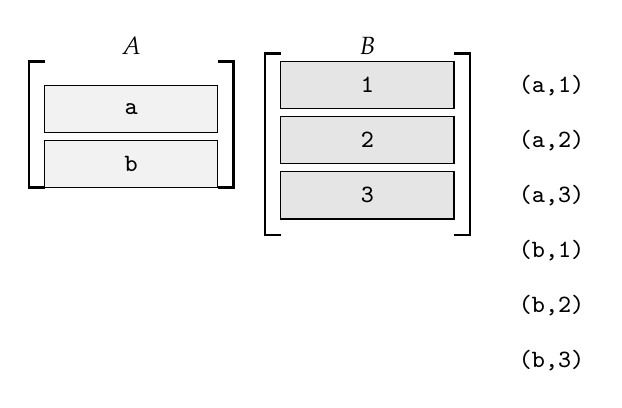
\begin{tikzpicture}[
			cell/.style={rectangle, draw=black, minimum width=2.2cm, minimum height=0.6cm, align=center, font=\ttfamily\small},
			hdr/.style={font=\sffamily\small}
		]
		\node[hdr] at (-2.5, 1.1) {$A$};
		\node[hdr] at (0.5, 1.1) {$B$};
		\node[cell, fill=black!5] at (-2.5, 0.3) {a};
		\node[cell, fill=black!5] at (-2.5, -0.4) {b};
		\node[cell, fill=black!10] at (0.5, 0.6) {1};
		\node[cell, fill=black!10] at (0.5, -0.1) {2};
		\node[cell, fill=black!10] at (0.5, -0.8) {3};
		\node[font=\ttfamily\small, anchor=west] at (2.3, 0.6) {(a,1)};
		\node[font=\ttfamily\small, anchor=west] at (2.3, -0.1) {(a,2)};
		\node[font=\ttfamily\small, anchor=west] at (2.3, -0.8) {(a,3)};
		\node[font=\ttfamily\small, anchor=west] at (2.3, -1.5) {(b,1)};
		\node[font=\ttfamily\small, anchor=west] at (2.3, -2.2) {(b,2)};
		\node[font=\ttfamily\small, anchor=west] at (2.3, -2.9) {(b,3)};

		\draw[thick] (-3.6, 0.9) -- (-3.8, 0.9) -- (-3.8, -0.7) -- (-3.6, -0.7);
		\draw[thick] (-1.4, 0.9) -- (-1.2, 0.9) -- (-1.2, -0.7) -- (-1.4, -0.7);
		\draw[thick] (-0.6, 1.0) -- (-0.8, 1.0) -- (-0.8, -1.3) -- (-0.6, -1.3);
		\draw[thick] (1.6, 1.0) -- (1.8, 1.0) -- (1.8, -1.3) -- (1.6, -1.3);
	\end{tikzpicture}
	\caption{Perkalian kartesian $A \times B$ dengan $|A|=2$ dan $|B|=3$ menghasilkan enam pasangan berurutan.}
	\label{fig:kartesian}
\end{figure}

Cara membaca Gambar~\ref{fig:kartesian}: gambar ini terdiri dari tiga kolom yang dipisahkan oleh tanda kurung siku matriks. Kolom kiri adalah himpunan $A$ dan berisi dua kotak kecil dari atas ke bawah: a dan b. Kolom tengah adalah himpunan $B$ dan berisi tiga kotak kecil dari atas ke bawah: 1, 2, dan 3. Kolom kanan adalah hasil perkalian kartesian berupa daftar enam pasangan berurutan yang tersusun tiga baris dua tingkat, yaitu (a,1), (a,2), (a,3), lalu (b,1), (b,2), (b,3). Setiap elemen $A$ dipasangkan tepat satu kali dengan setiap elemen $B$. Tidak ada pasangan yang terlewat. Kotak $A$ memakai latar abu-abu sangat muda dan kotak $B$ memakai latar abu-abu yang sedikit lebih gelap supaya asal komponen mudah dibedakan. Inti pesan gambar ini adalah perkalian kartesian menghasilkan seluruh kombinasi yang mungkin antara dua himpunan, dan jumlahnya adalah hasil kali kardinalitas masing-masing.

\subsection{Cara Berpikir: Membaca Notasi Perkalian Kartesian}

Saat membaca notasi $A \times B$, arahkan mata ke komponen pertama di dalam kurung. Komponen pertama selalu diambil dari himpunan kiri. Komponen kedua selalu diambil dari himpunan kanan. Jika penulis membalik urutan menjadi $B \times A$, artinya himpunan kanan sekarang menjadi sumber komponen pertama, sehingga hasilnya berbeda.

Untuk memeriksa apakah dua pasangan berurutan sama, bandingkan komponen pertama dahulu. Jika komponen pertama berbeda, kedua pasangan sudah pasti berbeda, walaupun komponen keduanya mirip. Jika komponen pertama sama, baru bandingkan komponen kedua.

\subsection{Kalau Salah: Membalik Urutan Komponen}

Kesalahan paling sering adalah mengira $A \times B$ sama dengan $B \times A$. Keduanya berbeda. Dengan $A=\{a,b\}$ dan $B=\{1,2,3\}$, hasil $A \times B$ memuat $(a,1)$ tetapi $B \times A$ memuat $(1,a)$. Kedua pasangan itu tidak sama, karena urutan komponennya berbeda.

Dalam basis data, kesalahan ini muncul sebagai tertukarnya kolom pada tabel. Jika tabel KRS menyimpan $(mahasiswa, matakuliah)$ tetapi query membacanya sebagai $(matakuliah, mahasiswa)$, maka filter "mahasiswa yang mengambil MTK" akan mencari di kolom yang salah. Hasilnya kosong, walaupun data sebenarnya ada.

\subsection{Mengapa Ini Penting untuk Rekayasa Perangkat Lunak}

Perkalian kartesian adalah bahan dasar relasi. Setiap relasi adalah himpunan bagian dari perkalian kartesian. Tanpa memahami perkalian kartesian, pengembang tidak bisa menjelaskan mengapa relasi $R$ harus merupakan subset dari $A \times B$.

Di basis data, perkalian kartesian setara dengan CROSS JOIN. Query yang secara tidak sengaja melakukan CROSS JOIN akan menghasilkan tabel raksasa. Jika tabel $A$ berisi 10 ribu baris dan tabel $B$ berisi 10 ribu baris, hasilnya seratus juta baris. Mengetahui bahwa operasi ini tumbuh secara perkalian, bukan penjumlahan, membuat pengembang waspada terhadap query yang lambat.

\subsection{Ringkasan}

Tabel~\ref{tab:kartesian} merangkum perkalian kartesian.

\begin{table}[H]
	\centering
	\caption{Ringkasan perkalian kartesian.}
	\label{tab:kartesian}
	\small
	\begin{tabularx}{\textwidth}{l X}
		\toprule
		Aspek            & Isi                                          \\
		\midrule
		Notasi           & $A \times B=\{(a,b) \mid a \in A, b \in B\}$ \\
		Komponen pertama & selalu dari $A$                              \\
		Komponen kedua   & selalu dari $B$                              \\
		Kardinalitas     & $|A \times B|=|A| \cdot |B|$                 \\
		Urutan komponen  & bermakna, $(a,b) \ne (b,a)$                  \\
		Padanan SQL      & CROSS JOIN                                   \\
		\bottomrule
	\end{tabularx}
\end{table}

\section{Definisi Relasi}

\subsection{Analogi: Daftar Pasangan di KRS}

Portal KRS tidak menyimpan seluruh kemungkinan pasangan mahasiswa dan mata kuliah. Ia hanya menyimpan pasangan yang benar-benar terjadi. Dari enam kemungkinan pasangan antara tiga mahasiswa dan dua mata kuliah, hanya mungkin empat pasangan yang benar-benar diambil pada semester ini. Empat pasangan itulah yang menjadi relasi.

Relasi adalah himpunan bagian dari perkalian kartesian yang memenuhi syarat tertentu. Syarat itulah yang menentukan pasangan mana yang masuk dan mana yang tidak.

\subsection{Definisi Formal}

Relasi $R$ dari himpunan $A$ ke himpunan $B$ adalah himpunan bagian dari $A \times B$. Notasinya $R \subseteq A \times B$. Himpunan $A$ disebut domain, himpunan $B$ disebut kodomain, dan himpunan semua komponen kedua yang benar-benar muncul disebut range \cite{rosen}.

Contoh: dengan $A=\{a,b\}$ dan $B=\{1,2,3\}$, ambil relasi $R=\{(a,1),(b,3)\}$. Relasi $R$ adalah himpunan bagian dari $A \times B$ dengan dua anggota. Anggota lain dari $A \times B$, misalnya $(a,2)$, $(a,3)$, $(b,1)$, $(b,2)$, tidak termasuk dalam $R$. Anggota $R$ hanya pasangan yang memenuhi syarat.

\subsection{Mengapa Ini Penting}

Basis data relasional memakai istilah relasi untuk tabel. Setiap baris tabel adalah satu pasangan berurutan. Setiap tabel adalah himpunan bagian dari perkalian kartesian kolom-kolomnya. Ketika pengembang menulis CHECK CONSTRAINT, ia sedang menetapkan syarat keanggotaan relasi. Ketika pengembang menulis UNIQUE CONSTRAINT, ia sedang menjamin bahwa setiap pasangan dalam relasi berbeda dari yang lain \cite{date}.

\subsection{Cara Berpikir: Memeriksa Apakah R adalah Relasi}

Untuk memeriksa apakah $R$ adalah relasi dari $A$ ke $B$, ajukan dua pertanyaan berurutan. Pertama, apakah setiap anggota $R$ berbentuk pasangan berurutan $(a,b)$ dengan $a \in A$ dan $b \in B$? Jika ada anggota yang komponen pertamanya bukan elemen $A$, atau komponen keduanya bukan elemen $B$, maka $R$ bukan relasi dari $A$ ke $B$. Kedua, apakah $R$ adalah himpunan, artinya tidak memuat pasangan yang sama dua kali? Jika ada pasangan yang berulang, penulisan himpunan menghapus duplikat secara otomatis, sehingga hasil akhirnya tetap himpunan.

Jika kedua pertanyaan itu dijawab, $R$ adalah relasi. Jika salah satu dilanggar, $R$ bukan relasi.

\section{Representasi Relasi}

\subsection{Analogi: Tiga Cara Membaca Peta}

Peta bisa dibaca dalam tiga bentuk. Bentuk pertama adalah peta jalan dengan panah dari kota asal ke kota tujuan. Bentuk kedua adalah daftar perjalanan yang ditulis di buku: baris pertama menyebut asal dan tujuan, baris kedua menyebut asal dan tujuan berikutnya. Bentuk ketiga adalah tabel jarak dengan titik-titik pertemuan yang ditandai.

Ketiganya menyampaikan informasi yang sama, tetapi dipakai untuk keperluan yang berbeda. Peta jalan paling baik untuk melihat arah. Daftar perjalanan paling baik untuk dibaca berurutan. Tabel jarak paling baik untuk diolah komputer.

Relasi juga punya tiga representasi serupa: diagram panah, tabel, dan matriks biner.

\subsection{Diagram Panah}

Diagram panah menampilkan dua himpunan sebagai dua daerah, dengan panah dari elemen asal ke elemen tujuan untuk setiap pasangan yang termasuk relasi. Perhatikan Gambar~\ref{fig:panah}.

\begin{figure}[H]
	\centering
	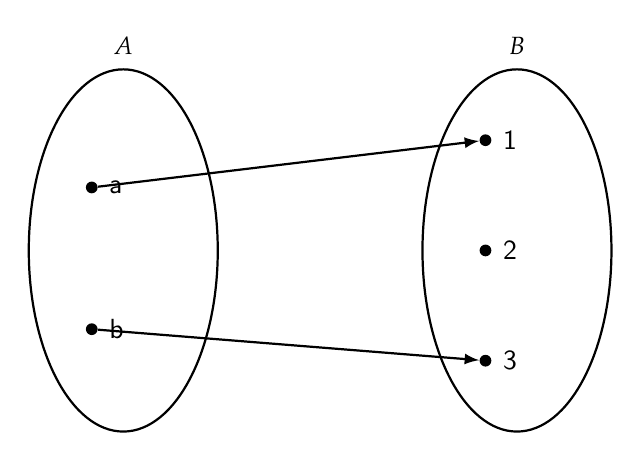
\begin{tikzpicture}[
			dot/.style={circle, fill=black, inner sep=1.5pt},
			dlbl/.style={font=\sffamily\small},
			elbl/.style={font=\sffamily}
		]
		\draw[thick] (-2, 0) ellipse (1.2 and 2.3);
		\draw[thick] (3, 0) ellipse (1.2 and 2.3);
		\node[dlbl] at (-2, 2.6) {$A$};
		\node[dlbl] at (3, 2.6) {$B$};

		\node[dot] (a) at (-2.4, 0.8) {};
		\node[dot] (b) at (-2.4, -1.0) {};
		\node[elbl, anchor=west] at (-2.3, 0.8) {a};
		\node[elbl, anchor=west] at (-2.3, -1.0) {b};

		\node[dot] (n1) at (2.6, 1.4) {};
		\node[dot] (n2) at (2.6, 0) {};
		\node[dot] (n3) at (2.6, -1.4) {};
		\node[elbl, anchor=west] at (2.7, 1.4) {1};
		\node[elbl, anchor=west] at (2.7, 0) {2};
		\node[elbl, anchor=west] at (2.7, -1.4) {3};

		\draw[thick, -latex] (a) -- (n1);
		\draw[thick, -latex] (b) -- (n3);
	\end{tikzpicture}
	\caption{Diagram panah relasi $R=\{(a,1),(b,3)\}$ dari $A$ ke $B$.}
	\label{fig:panah}
\end{figure}

Cara membaca Gambar~\ref{fig:panah}: gambar ini menampilkan dua elips berdampingan. Elips kiri berlabel $A$ di atas dan berisi dua titik hitam berlabel a dan b dari atas ke bawah. Elips kanan berlabel $B$ di atas dan berisi tiga titik hitam berlabel 1, 2, dan 3 dari atas ke bawah. Ada dua panah. Panah pertama bergerak dari titik a menuju titik 1. Panah kedua bergerak dari titik b menuju titik 3. Titik a tidak punya panah ke 2 atau 3. Titik b tidak punya panah ke 1 atau 2. Titik 2 tidak punya panah dari a maupun b. Inti pesan gambar ini adalah diagram panah menunjukkan arah hubungan secara visual, dan elemen yang tidak punya panah berarti tidak terhubung.

\subsection{Tabel}

Tabel menampilkan pasangan sebagai baris. Kolom pertama berisi elemen domain, kolom kedua berisi elemen kodomain. Relasi $R=\{(a,1),(b,3)\}$ ditampilkan pada Tabel~\ref{tab:relasi-tabel}.

\begin{table}[H]
	\centering
	\caption{Representasi relasi $R$ sebagai tabel.}
	\label{tab:relasi-tabel}
	\small
	\begin{tabular}{c c}
		\toprule
		$A$ & $B$ \\
		\midrule
		a   & 1   \\
		b   & 3   \\
		\bottomrule
	\end{tabular}
\end{table}

Tabel itu menyampaikan informasi yang sama dengan diagram panah, tetapi dalam bentuk yang lebih mudah dibaca mesin. Setiap baris adalah satu tuple di basis data relasional. Kolom pertama disebut foreign key ke tabel $A$, kolom kedua disebut foreign key ke tabel $B$.

\subsection{Matriks Biner}

Matriks biner menampilkan relasi sebagai matriks yang berisi hanya angka 0 dan 1. Baris mewakili elemen domain, kolom mewakili elemen kodomain. Elemen $m_{ij}=1$ jika $(a_i,b_j) \in R$, dan $m_{ij}=0$ jika $(a_i,b_j) \notin R$ \cite{rosen}.

Untuk relasi $R=\{(a,1),(b,3)\}$ dengan $A=\{a,b\}$ dan $B=\{1,2,3\}$, matriks binernya adalah $\begin{bmatrix}1&0&0\\0&0&1\end{bmatrix}$. Baris pertama untuk $a$, baris kedua untuk $b$. Kolom pertama untuk 1, kolom kedua untuk 2, kolom ketiga untuk 3. Angka 1 muncul di posisi $(1,1)$ dan $(2,3)$ karena $(a,1)$ dan $(b,3)$ termasuk relasi. Posisi lain berisi 0.

\subsection{Tiga Representasi Berdampingan}

Perhatikan Gambar~\ref{fig:tiga-representasi} yang menyandingkan ketiga representasi dalam satu pandangan.

\begin{figure}[H]
	\centering
	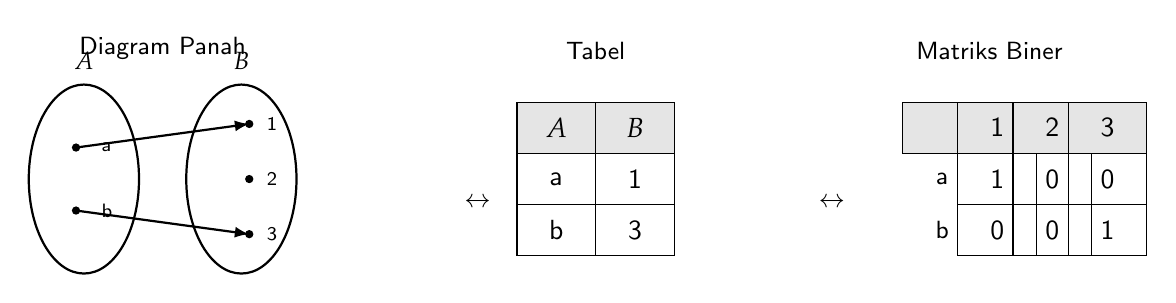
\begin{tikzpicture}[
			cell/.style={rectangle, draw=black, minimum width=1.0cm, minimum height=0.65cm, align=center, font=\sffamily},
			lbl/.style={font=\sffamily\small}
		]
		\node[font=\sffamily\small, anchor=south] at (0, 1.4) {Diagram Panah};
		\draw[thick] (-1.0, 0) ellipse (0.7 and 1.2);
		\draw[thick] (1.0, 0) ellipse (0.7 and 1.2);
		\node[lbl] at (-1.0, 1.5) {$A$};
		\node[lbl] at (1.0, 1.5) {$B$};
		\fill (-1.1, 0.4) circle (1.5pt);
		\fill (-1.1, -0.4) circle (1.5pt);
		\fill (1.1, 0.7) circle (1.5pt);
		\fill (1.1, 0) circle (1.5pt);
		\fill (1.1, -0.7) circle (1.5pt);
		\node[font=\scriptsize\sffamily, anchor=west] at (-0.9, 0.4) {a};
		\node[font=\scriptsize\sffamily, anchor=west] at (-0.9, -0.4) {b};
		\node[font=\scriptsize\sffamily, anchor=west] at (1.2, 0.7) {1};
		\node[font=\scriptsize\sffamily, anchor=west] at (1.2, 0) {2};
		\node[font=\scriptsize\sffamily, anchor=west] at (1.2, -0.7) {3};
		\draw[thick, -latex] (-1.1, 0.4) -- (1.1, 0.7);
		\draw[thick, -latex] (-1.1, -0.4) -- (1.1, -0.7);

		\node[font=\sffamily\small, anchor=south] at (5.5, 1.4) {Tabel};
		\node[cell, fill=black!10] at (5.0, 0.65) {$A$};
		\node[cell, fill=black!10] at (6.0, 0.65) {$B$};
		\node[cell] at (5.0, 0) {a};
		\node[cell] at (6.0, 0) {1};
		\node[cell] at (5.0, -0.65) {b};
		\node[cell] at (6.0, -0.65) {3};

		\node[font=\sffamily\small, anchor=south] at (10.5, 1.4) {Matriks Biner};
		\node[cell, fill=black!10] at (9.9, 0.65) {};
		\node[cell, fill=black!10] at (10.6, 0.65) {1};
		\node[cell, fill=black!10] at (11.3, 0.65) {2};
		\node[cell, fill=black!10] at (12.0, 0.65) {3};
		\node[lbl] at (9.9, 0) {a};
		\node[cell] at (10.6, 0) {1};
		\node[cell] at (11.3, 0) {0};
		\node[cell] at (12.0, 0) {0};
		\node[lbl] at (9.9, -0.65) {b};
		\node[cell] at (10.6, -0.65) {0};
		\node[cell] at (11.3, -0.65) {0};
		\node[cell] at (12.0, -0.65) {1};

		\node[font=\sffamily\small] at (4.0, -0.3) {$\leftrightarrow$};
		\node[font=\sffamily\small] at (8.5, -0.3) {$\leftrightarrow$};
	\end{tikzpicture}
	\caption{Tiga representasi relasi $R=\{(a,1),(b,3)\}$.}
	\label{fig:tiga-representasi}
\end{figure}

Cara membaca Gambar~\ref{fig:tiga-representasi}: gambar ini menampilkan tiga panel dari kiri ke kanan yang dihubungkan oleh tanda panah bolak-balik. Panel pertama berjudul "Diagram Panah" dan menampilkan dua elips dengan titik-titik dan panah seperti pada gambar sebelumnya. Panel kedua berjudul "Tabel" dan menampilkan kotak dua baris dua kolom dengan header $A$ dan $B$, serta isi a-1 di baris pertama dan b-3 di baris kedua. Panel ketiga berjudul "Matriks Biner" dan menampilkan kotak dua baris empat kolom dengan header 1, 2, 3, dan label baris a, b, dengan isi 1-0-0 di baris pertama dan 0-0-1 di baris kedua. Tanda panah bolak-balik di antara panel menandakan bahwa ketiga representasi menyampaikan informasi yang sama. Inti pesan gambar ini adalah satu relasi bisa disajikan dalam tiga cara, dan pilihan cara bergantung pada keperluan pembaca.

\subsection{Kalau Salah: Matriks Biner Dikira Matriks Biasa}

Matriks biner hanyalah alat penyajian. Operasi yang lazim pada matriks biasa, misalnya determinan atau invers, tidak otomatis bermakna pada matriks biner. Determinan matriks biner bisa saja bernilai 0 atau bukan bilangan bulat, dan hasil itu tidak memiliki tafsiran relasional. Yang bermakna pada matriks biner adalah posisi angka 1, bukan nilai numeriknya.

Kesalahan yang lebih halus adalah mengira matriks biner bisa dipakai untuk menghitung jarak antar entitas. Jarak dihitung dengan cara lain, bukan dengan determinan matriks biner.

\subsection{Mengapa Ini Penting}

Dalam basis data relasional, ketiga representasi punya padanan langsung. Diagram panah setara dengan diagram relasi antar tabel. Tabel setara dengan tabel fisik di database. Matriks biner setara dengan matriks keputusan yang dipakai saat merancang indeks. Pengembang yang mengenali ketiga padanan ini dapat berpindah antara desain konseptual, implementasi fisik, dan optimasi tanpa bingung \cite{date}.

\subsection{Ringkasan}

Tabel~\ref{tab:representasi} merangkum tiga representasi.

\begin{table}[H]
	\centering
	\caption{Perbandingan tiga representasi relasi.}
	\label{tab:representasi}
	\small
	\begin{tabularx}{\textwidth}{l X X}
		\toprule
		Representasi  & Kelebihan              & Kekurangan                 \\
		\midrule
		Diagram panah & arah langsung terlihat & sulit dibaca mesin         \\
		Tabel         & mudah dibaca manusia   & hanya dua kolom            \\
		Matriks biner & mudah diolah komputer  & hanya untuk himpunan kecil \\
		\bottomrule
	\end{tabularx}
\end{table}

\section{Sifat-Sifat Relasi}

\subsection{Analogi: Empat Pertanyaan Tentang Hubungan}

Sebuah relasi pada himpunan $A$ punya empat pertanyaan yang harus dijawab. Pertama, apakah setiap elemen terhubung dengan dirinya sendiri? Kedua, apakah setiap rantai dua langkah dapat dipendekkan menjadi satu langkah? Ketiga, apakah setiap panah punya panah balik? Keempat, apakah panah balik hanya muncul ketika kedua ujungnya adalah elemen yang sama?

Keempat pertanyaan itu masing-masing menghasilkan satu sifat: refleksif, menghantar, setangkup, dan tolak-setangkup \cite{rosen}.

\subsection{Refleksif}

Relasi $R$ pada himpunan $A$ disebut refleksif jika untuk setiap $a \in A$, berlaku $(a,a) \in R$. Dengan kata lain, setiap elemen terhubung dengan dirinya sendiri. Relasi tidak refleksif jika ada minimal satu $a \in A$ sehingga $(a,a) \notin R$.

Pada matriks biner, refleksif terlihat dari diagonal utama. Jika semua elemen diagonal utama bernilai 1, relasi refleksif. Jika ada satu saja diagonal utama yang bernilai 0, relasi tidak refleksif. Perhatikan Gambar~\ref{fig:refleksif}.

\begin{figure}[H]
	\centering
	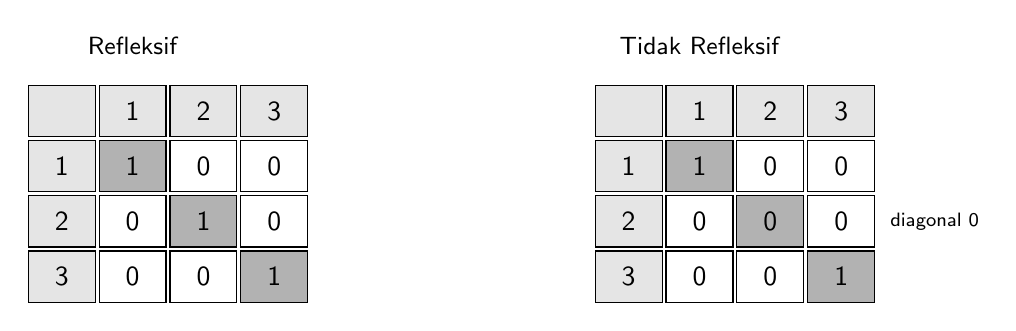
\begin{tikzpicture}[
			cell/.style={rectangle, draw=black, minimum width=0.85cm, minimum height=0.65cm, align=center, font=\sffamily},
			hl/.style={cell, fill=black!30}
		]
		\node[font=\sffamily\small, anchor=south] at (1.3, 1.6) {Refleksif};
		\node[cell, fill=black!10] at (0.4, 1.0) {};
		\node[cell, fill=black!10] at (1.3, 1.0) {1};
		\node[cell, fill=black!10] at (2.2, 1.0) {2};
		\node[cell, fill=black!10] at (3.1, 1.0) {3};
		\node[cell, fill=black!10] at (0.4, 0.3) {1};
		\node[hl] at (1.3, 0.3) {1};
		\node[cell] at (2.2, 0.3) {0};
		\node[cell] at (3.1, 0.3) {0};
		\node[cell, fill=black!10] at (0.4, -0.4) {2};
		\node[cell] at (1.3, -0.4) {0};
		\node[hl] at (2.2, -0.4) {1};
		\node[cell] at (3.1, -0.4) {0};
		\node[cell, fill=black!10] at (0.4, -1.1) {3};
		\node[cell] at (1.3, -1.1) {0};
		\node[cell] at (2.2, -1.1) {0};
		\node[hl] at (3.1, -1.1) {1};

		\node[font=\sffamily\small, anchor=south] at (8.5, 1.6) {Tidak Refleksif};
		\node[cell, fill=black!10] at (7.6, 1.0) {};
		\node[cell, fill=black!10] at (8.5, 1.0) {1};
		\node[cell, fill=black!10] at (9.4, 1.0) {2};
		\node[cell, fill=black!10] at (10.3, 1.0) {3};
		\node[cell, fill=black!10] at (7.6, 0.3) {1};
		\node[hl] at (8.5, 0.3) {1};
		\node[cell] at (9.4, 0.3) {0};
		\node[cell] at (10.3, 0.3) {0};
		\node[cell, fill=black!10] at (7.6, -0.4) {2};
		\node[cell] at (8.5, -0.4) {0};
		\node[hl] at (9.4, -0.4) {0};
		\node[cell] at (10.3, -0.4) {0};
		\node[cell, fill=black!10] at (7.6, -1.1) {3};
		\node[cell] at (8.5, -1.1) {0};
		\node[cell] at (9.4, -1.1) {0};
		\node[hl] at (10.3, -1.1) {1};

		\node[font=\scriptsize\sffamily, anchor=west] at (10.8, -0.4) {diagonal 0};
	\end{tikzpicture}
	\caption{Cek refleksif dari diagonal utama matriks biner.}
	\label{fig:refleksif}
\end{figure}

Cara membaca Gambar~\ref{fig:refleksif}: gambar ini menampilkan dua matriks biner berdampingan. Matriks kiri berjudul "Refleksif" dan memiliki diagonal utama berisi 1-1-1. Sel-sel diagonal itu diberi latar abu-abu gelap untuk menonjolkan. Matriks kanan berjudul "Tidak Refleksif" dan memiliki diagonal utama 1-0-1. Sel diagonal kedua yang bernilai 0 diberi latar abu-abu lebih gelap dan di sebelah kanan ada keterangan "diagonal 0". Inti pesan gambar ini adalah refleksif dapat dibaca sekilas dari diagonal utama, dan satu angka 0 saja sudah cukup untuk menggugurkan sifat itu.

\subsection{Menghantar}

Relasi $R$ pada himpunan $A$ disebut menghantar jika setiap kali $(a,b) \in R$ dan $(b,c) \in R$, maka $(a,c) \in R$. Dengan kata lain, rantai dua langkah dapat dipendekkan menjadi satu langkah tanpa keluar dari relasi. Perhatikan Gambar~\ref{fig:menghantar}.

\begin{figure}[H]
	\centering
	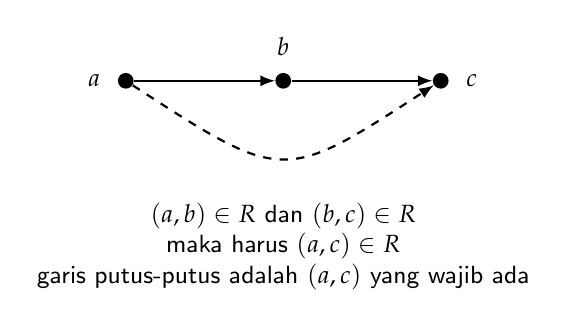
\begin{tikzpicture}[
			dot/.style={circle, fill=black, inner sep=2pt},
			lbl/.style={font=\sffamily\small}
		]
		\node[dot] (a) at (0, 1.5) {};
		\node[lbl, anchor=east] at (-0.2, 1.5) {$a$};
		\node[dot] (b) at (2, 1.5) {};
		\node[lbl, anchor=south] at (2, 1.7) {$b$};
		\node[dot] (c) at (4, 1.5) {};
		\node[lbl, anchor=west] at (4.2, 1.5) {$c$};

		\draw[thick, -latex] (a) -- (b);
		\draw[thick, -latex] (b) -- (c);
		\draw[thick, dashed, -latex] (a) .. controls (2, 0.2) .. (c);

		\node[font=\small\sffamily, align=center] at (2, -0.6) {
			$(a,b) \in R$ dan $(b,c) \in R$\\
			maka harus $(a,c) \in R$\\
			garis putus-putus adalah $(a,c)$ yang wajib ada
		};
	\end{tikzpicture}
	\caption{Syarat menghantar: rantai dua langkah harus bisa dipendekkan menjadi satu langkah.}
	\label{fig:menghantar}
\end{figure}

Cara membaca Gambar~\ref{fig:menghantar}: gambar ini menampilkan tiga titik hitam berderet dari kiri ke kanan, berlabel $a$, $b$, dan $c$. Ada panah penuh dari $a$ ke $b$ dan panah penuh dari $b$ ke $c$. Di bawah dua panah itu ada garis putus-putus yang melengkung dari $a$ langsung ke $c$. Di bawah gambar ada keterangan bahwa jika dua panah penuh ada, panah putus-putus wajib ada. Inti pesan gambar ini adalah menghantar berarti rantai tidak boleh menganga, setiap jalan pintas harus tersedia.

\subsection{Setangkup dan Tolak-setangkup}

Relasi $R$ pada himpunan $A$ disebut setangkup jika setiap kali $(a,b) \in R$, maka $(b,a) \in R$. Dengan kata lain, setiap panah punya panah balik.

Relasi $R$ pada himpunan $A$ disebut tolak-setangkup jika setiap kali $(a,b) \in R$ dan $(b,a) \in R$, maka $a=b$. Dengan kata lain, panah balik hanya boleh muncul untuk elemen yang sama.

Perhatikan bahwa setangkup dan tolak-setangkup adalah dua sifat yang berbeda, bukan dua sisi dari satu koin. Sebuah relasi bisa setangkup, tolak-setangkup, keduanya, atau tidak keduanya. Perhatikan Gambar~\ref{fig:setangkup}.

\begin{figure}[H]
	\centering
	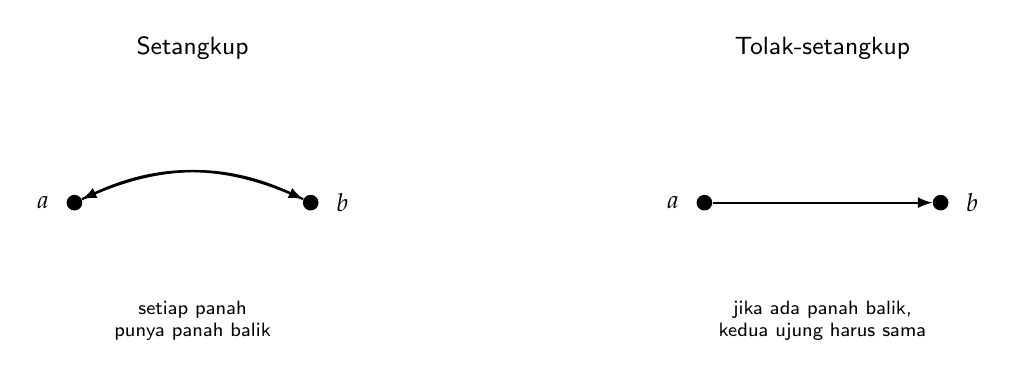
\begin{tikzpicture}[
			dot/.style={circle, fill=black, inner sep=2pt},
			lbl/.style={font=\sffamily\small},
			hdr/.style={font=\sffamily\small, anchor=south}
		]
		\begin{scope}[shift={(-4.5, 0)}]
			\node[hdr] at (1.5, 2.2) {Setangkup};
			\node[dot] (a) at (0, 0.5) {};
			\node[lbl, anchor=east] at (-0.2, 0.5) {$a$};
			\node[dot] (b) at (3, 0.5) {};
			\node[lbl, anchor=west] at (3.2, 0.5) {$b$};
			\draw[thick, -latex, bend left=25] (a) to (b);
			\draw[thick, -latex, bend right=25] (b) to (a);
			\node[font=\scriptsize\sffamily, align=center] at (1.5, -1.0) {setiap panah\\punya panah balik};
		\end{scope}

		\begin{scope}[shift={(3.5, 0)}]
			\node[hdr] at (1.5, 2.2) {Tolak-setangkup};
			\node[dot] (a) at (0, 0.5) {};
			\node[lbl, anchor=east] at (-0.2, 0.5) {$a$};
			\node[dot] (b) at (3, 0.5) {};
			\node[lbl, anchor=west] at (3.2, 0.5) {$b$};
			\draw[thick, -latex] (a) -- (b);
			\node[font=\scriptsize\sffamily, align=center] at (1.5, -1.0) {jika ada panah balik,\\kedua ujung harus sama};
		\end{scope}
	\end{tikzpicture}
	\caption{Perbandingan sifat setangkup dan tolak-setangkup.}
	\label{fig:setangkup}
\end{figure}

Cara membaca Gambar~\ref{fig:setangkup}: gambar ini menampilkan dua subgambar berdampingan. Subgambar kiri berjudul "Setangkup" dan menampilkan dua titik $a$ dan $b$ yang dihubungkan oleh dua panah berlawanan arah, satu melengkung di atas dan satu melengkung di bawah. Di bawah subgambar ada keterangan bahwa setiap panah punya panah balik. Subgambar kanan berjudul "Tolak-setangkup" dan menampilkan dua titik $a$ dan $b$ yang dihubungkan hanya oleh satu panah dari $a$ ke $b$, tanpa panah balik. Di bawah subgambar ada keterangan bahwa jika ada panah balik, kedua ujungnya harus sama. Inti pesan gambar ini adalah setangkup memperbolehkan panah balik antar elemen berbeda, sedangkan tolak-setangkup melarangnya.

\subsection{Tiga Contoh Relasi dengan Matriks}

Tiga contoh relasi pada himpunan $A=\{1,2,3\}$ disajikan pada Gambar~\ref{fig:tiga-matriks-sifat}. Ketiga contoh itu menunjukkan bahwa sifat relasi bisa dikombinasikan dengan cara yang berbeda-beda.

\begin{figure}[H]
	\centering
	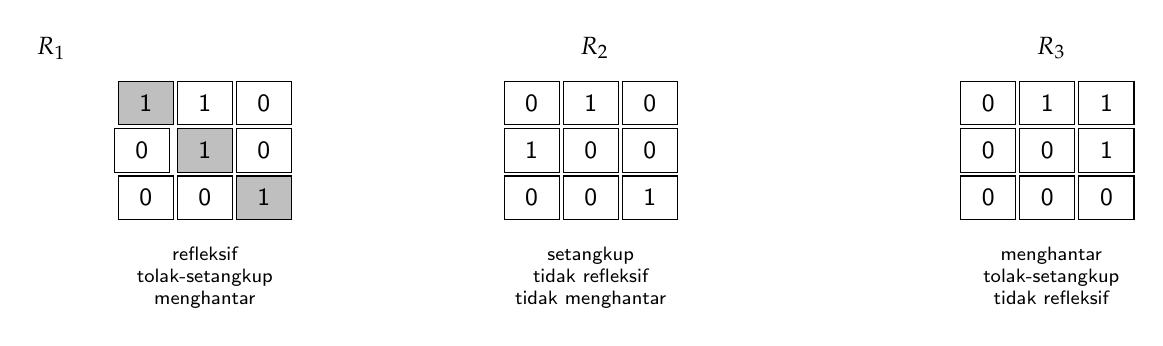
\begin{tikzpicture}[
			cell/.style={rectangle, draw=black, minimum width=0.7cm, minimum height=0.55cm, align=center, font=\small\sffamily},
			diag/.style={cell, fill=black!25},
			hdr/.style={font=\sffamily\small}
		]
		\node[hdr] at (-1.2, 2.5) {$R_1$};
		\node[diag] at (0, 1.8) {1};
		\node[cell] at (0.75, 1.8) {1};
		\node[cell] at (1.5, 1.8) {0};
		\node[cell] at (-0.05, 1.2) {0};
		\node[diag] at (0.75, 1.2) {1};
		\node[cell] at (1.5, 1.2) {0};
		\node[cell] at (0, 0.6) {0};
		\node[cell] at (0.75, 0.6) {0};
		\node[diag] at (1.5, 0.6) {1};
		\node[font=\scriptsize\sffamily, anchor=north, align=center] at (0.75, 0.1) {refleksif\\tolak-setangkup\\menghantar};

		\node[hdr] at (5.7, 2.5) {$R_2$};
		\node[cell] at (4.9, 1.8) {0};
		\node[cell] at (5.65, 1.8) {1};
		\node[cell] at (6.4, 1.8) {0};
		\node[cell] at (4.9, 1.2) {1};
		\node[cell] at (5.65, 1.2) {0};
		\node[cell] at (6.4, 1.2) {0};
		\node[cell] at (4.9, 0.6) {0};
		\node[cell] at (5.65, 0.6) {0};
		\node[cell] at (6.4, 0.6) {1};
		\node[font=\scriptsize\sffamily, anchor=north, align=center] at (5.65, 0.1) {setangkup\\tidak refleksif\\tidak menghantar};

		\node[hdr] at (11.5, 2.5) {$R_3$};
		\node[cell] at (10.7, 1.8) {0};
		\node[cell] at (11.45, 1.8) {1};
		\node[cell] at (12.2, 1.8) {1};
		\node[cell] at (10.7, 1.2) {0};
		\node[cell] at (11.45, 1.2) {0};
		\node[cell] at (12.2, 1.2) {1};
		\node[cell] at (10.7, 0.6) {0};
		\node[cell] at (11.45, 0.6) {0};
		\node[cell] at (12.2, 0.6) {0};
		\node[font=\scriptsize\sffamily, anchor=north, align=center] at (11.5, 0.1) {menghantar\\tolak-setangkup\\tidak refleksif};
	\end{tikzpicture}
	\caption{Tiga contoh relasi dengan matriks dan sifat masing-masing.}
	\label{fig:tiga-matriks-sifat}
\end{figure}

Cara membaca Gambar~\ref{fig:tiga-matriks-sifat}: gambar ini menampilkan tiga matriks biner berdampingan dari kiri ke kanan. Matriks $R_1$ memiliki diagonal utama 1-1-1 yang ditandai dengan latar abu-abu gelap, dan satu angka 1 tambahan di luar diagonal pada posisi baris 1 kolom 2. Di bawahnya tertulis sifat refleksif, tolak-setangkup, dan menghantar. Matriks $R_2$ memiliki angka 1 pada posisi (1,2) dan (2,1) yang saling bercermin, serta posisi (3,3). Diagonal utamanya 0-0-1 sehingga tidak refleksif. Di bawahnya tertulis sifat setangkup, tidak refleksif, dan tidak menghantar. Matriks $R_3$ memiliki angka 1 pada posisi (1,2), (1,3), dan (2,3) yang membentuk rantai tanpa balik. Di bawahnya tertulis sifat menghantar, tolak-setangkup, dan tidak refleksif. Inti pesan gambar ini adalah setiap matriks menunjukkan kombinasi sifat yang berbeda, dan kombinasi itu bisa dibaca langsung dari pola angka 1 di dalam matriks.

\subsection{Menguji Sifat dari Contoh}

Perhatikan relasi $R=\{(1,1),(2,2),(2,3),(3,2),(4,2),(4,4)\}$. Relasi ini tidak setangkup karena $(4,2) \in R$ tetapi $(2,4) \notin R$. Relasi ini juga tidak tolak-setangkup karena $(2,3) \in R$ dan $(3,2) \in R$ tetapi $2 \ne 3$. Contoh ini menunjukkan bahwa relasi bisa sekaligus tidak setangkup dan tidak tolak-setangkup \cite{rosen}.

\subsection{Cara Berpikir: Memeriksa Sifat Secara Berurutan}

Saat memeriksa sifat relasi, ajukan empat pertanyaan secara berurutan. Pertama, apakah semua diagonal utama berisi 1? Jika ya, refleksif. Kedua, apakah setiap rantai dua langkah punya jalan pintas? Jika ya, menghantar. Ketiga, apakah setiap panah punya panah balik? Jika ya, setangkup. Keempat, apakah setiap panah balik hanya muncul pada elemen yang sama? Jika ya, tolak-setangkup.

Urutan pertanyaan ini tidak mengubah hasil, tetapi membantu agar tidak ada sifat yang terlewat. Setiap sifat adalah pemeriksaan terpisah, dan satu sifat tidak menggantikan sifat lain.

\subsection{Kalau Salah: Mengira Tidak Setangkup Sama dengan Tolak-setangkup}

Kesalahan paling sering adalah menganggap "tidak setangkup" dan "tolak-setangkup" sebagai dua nama untuk hal yang sama. Keduanya berbeda. Relasi bisa saja tidak setangkup tetapi juga tidak tolak-setangkup, seperti contoh $R=\{(1,1),(2,2),(2,3),(3,2),(4,2),(4,4)\}$ di atas.

Menganggap keduanya sama berbahaya saat merancang tabel basis data. Kolom yang seharusnya tolak-setangkup, misalnya nomor identitas, bisa diberi pasangan berulang jika pengembang mengira sudah aman karena "tidak setangkup". Akibatnya, dua baris bisa memiliki nomor identitas yang sama, dan sistem kehilangan integritas referensial.

\subsection{Mengapa Ini Penting}

Sifat relasi menentukan jenis constraint yang harus dipasang di basis data. Refleksif menentukan apakah foreign key boleh bernilai null atau tidak. Menghantar menentukan apakah relasi transitif harus ditutup secara eksplisit. Setangkup menentukan apakah indeks pada dua kolom perlu dikelola bersama. Tolak-setangkup menentukan apakah unique constraint harus dipasang. Tanpa memahami sifat relasi, pengembang memasang constraint secara sembarangan, dan sistem menjadi lambat atau tidak konsisten \cite{silberschatz}.

\subsection{Ringkasan}

Tabel~\ref{tab:sifat} merangkum keempat sifat.

\begin{table}[H]
	\centering
	\caption{Ringkasan empat sifat relasi.}
	\label{tab:sifat}
	\small
	\begin{tabularx}{\textwidth}{l X X}
		\toprule
		Sifat           & Syarat                                      & Cek matriks biner                     \\
		\midrule
		Refleksif       & $(a,a) \in R$ untuk semua $a$               & diagonal utama semua 1                \\
		Menghantar      & $(a,b),(b,c) \in R \Rightarrow (a,c) \in R$ & lihat rantai, periksa jalan pintas    \\
		Setangkup       & $(a,b) \in R \Rightarrow (b,a) \in R$       & $M=M^T$                               \\
		Tolak-setangkup & $(a,b),(b,a) \in R \Rightarrow a=b$         & di luar diagonal tidak ada pasangan 1 \\
		\bottomrule
	\end{tabularx}
\end{table}

\section{Relasi Invers}

\subsection{Analogi: Pertanyaan dari Arah Sebaliknya}

Portal KRS bisa menjawab dua pertanyaan dari data yang sama. Pertanyaan pertama: "M3 mengambil mata kuliah apa?" Pertanyaan kedua: "Siapa yang mengambil MTK?" Kedua jawaban berasal dari pasangan yang sama, hanya dibaca dari arah berbeda. Jawaban pertama membaca pasangan dari kiri ke kanan. Jawaban kedua membaca pasangan dari kanan ke kiri.

Relasi yang dibaca dari arah sebaliknya disebut relasi invers.

\subsection{Definisi Formal}

Jika $R$ adalah relasi dari himpunan $A$ ke himpunan $B$, maka invers $R^{-1}$ adalah relasi dari $B$ ke $A$ yang didefinisikan oleh $R^{-1}=\{(b,a) \mid (a,b) \in R\}$. Setiap pasangan dibalik urutannya \cite{rosen}.

Contoh: $R=\{(a,1),(b,3)\}$ memiliki $R^{-1}=\{(1,a),(3,b)\}$. Perhatikan bahwa elemen yang tadinya ada di kanan sekarang ada di kiri. Kumpulan pasangan tetap sama, hanya urutannya berubah. Perhatikan Gambar~\ref{fig:invers}.

\begin{figure}[H]
	\centering
	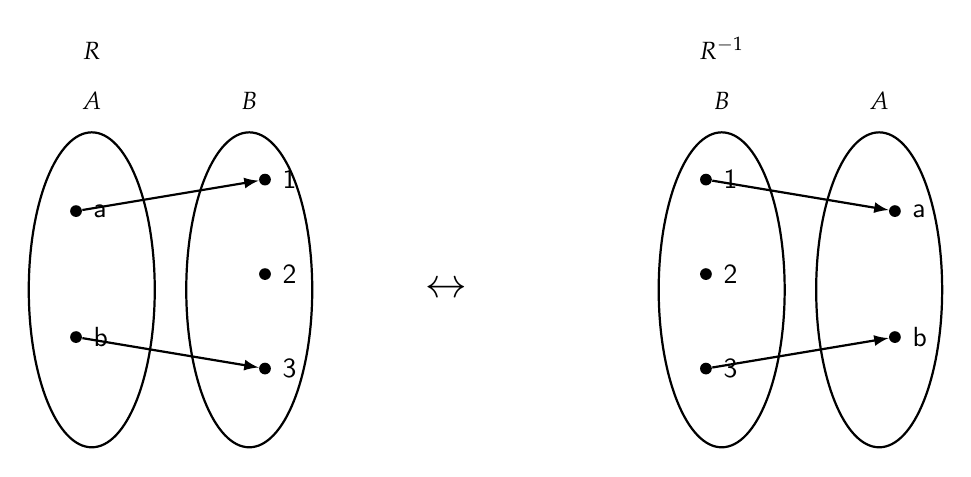
\begin{tikzpicture}[
			dot/.style={circle, fill=black, inner sep=1.5pt},
			lbl/.style={font=\sffamily\small},
			elbl/.style={font=\sffamily}
		]
		\begin{scope}[shift={(-3.5, 0)}]
			\node[lbl, anchor=south] at (-1, 2.8) {$R$};
			\draw[thick] (-1, 0) ellipse (0.8 and 2.0);
			\draw[thick] (1, 0) ellipse (0.8 and 2.0);
			\node[font=\sffamily\small] at (-1, 2.4) {$A$};
			\node[font=\sffamily\small] at (1, 2.4) {$B$};
			\node[dot] (a) at (-1.2, 1.0) {};
			\node[dot] (b) at (-1.2, -0.6) {};
			\node[elbl, anchor=west] at (-1.1, 1.0) {a};
			\node[elbl, anchor=west] at (-1.1, -0.6) {b};
			\node[dot] (n1) at (1.2, 1.4) {};
			\node[dot] (n2) at (1.2, 0.2) {};
			\node[dot] (n3) at (1.2, -1.0) {};
			\node[elbl, anchor=west] at (1.3, 1.4) {1};
			\node[elbl, anchor=west] at (1.3, 0.2) {2};
			\node[elbl, anchor=west] at (1.3, -1.0) {3};
			\draw[thick, -latex] (a) -- (n1);
			\draw[thick, -latex] (b) -- (n3);
		\end{scope}

		\node[font=\Large\sffamily] at (0, 0) {$\leftrightarrow$};

		\begin{scope}[shift={(4.5, 0)}]
			\node[lbl, anchor=south] at (-1, 2.8) {$R^{-1}$};
			\draw[thick] (-1, 0) ellipse (0.8 and 2.0);
			\draw[thick] (1, 0) ellipse (0.8 and 2.0);
			\node[font=\sffamily\small] at (-1, 2.4) {$B$};
			\node[font=\sffamily\small] at (1, 2.4) {$A$};
			\node[dot] (n1) at (-1.2, 1.4) {};
			\node[dot] (n2) at (-1.2, 0.2) {};
			\node[dot] (n3) at (-1.2, -1.0) {};
			\node[elbl, anchor=west] at (-1.1, 1.4) {1};
			\node[elbl, anchor=west] at (-1.1, 0.2) {2};
			\node[elbl, anchor=west] at (-1.1, -1.0) {3};
			\node[dot] (a) at (1.2, 1.0) {};
			\node[dot] (b) at (1.2, -0.6) {};
			\node[elbl, anchor=west] at (1.3, 1.0) {a};
			\node[elbl, anchor=west] at (1.3, -0.6) {b};
			\draw[thick, -latex] (n1) -- (a);
			\draw[thick, -latex] (n3) -- (b);
		\end{scope}
	\end{tikzpicture}
	\caption{Relasi $R$ dan inversnya $R^{-1}$: arah panah dibalik, posisi himpunan ditukar.}
	\label{fig:invers}
\end{figure}

Cara membaca Gambar~\ref{fig:invers}: gambar ini menampilkan dua subgambar yang dihubungkan tanda panah bolak-balik di tengah. Subgambar kiri berjudul $R$ dan menampilkan elips $A$ di kiri dan elips $B$ di kanan, dengan dua panah dari a ke 1 dan dari b ke 3. Subgambar kanan berjudul $R^{-1}$ dan menampilkan elips $B$ di kiri dan elips $A$ di kanan, dengan dua panah dari 1 ke a dan dari 3 ke b. Posisi elips ditukar dan arah panah dibalik. Isi himpunan tetap sama. Inti pesan gambar ini adalah invers relasi hanya membalik arah hubungan, bukan mengubah pasangan yang terhubung.

\subsection{Invers dalam Matriks}

Matriks relasi invers adalah transpos dari matriks relasi asli. Jika matriks asli $M=\begin{bmatrix}1&0&0\\0&0&1\end{bmatrix}$ berordo $2 \times 3$, maka matriks inversnya $M^T=\begin{bmatrix}1&0\\0&0\\0&1\end{bmatrix}$ berordo $3 \times 2$. Baris dan kolom bertukar posisi.

Perhatikan perbedaan penting. Transpos di sini adalah transpos relasi, bukan invers matriks seperti pada materi matriks. Invers matriks hanya ada jika determinannya bukan nol. Relasi invers selalu ada, karena setiap pasangan selalu bisa dibalik. Di KRS, $R_1$ berarti "mengambil" dan $R_1^{-1}$ berarti "diambil oleh" \cite{date}.

\subsection{Kalau Salah: Mengira Invers Relasi Sama dengan Invers Matriks}

Kesalahan paling sering adalah memakai lambang $R^{-1}$ dan mengira nilainya dihitung dengan rumus invers matriks $\frac{1}{\det(A)}\text{adj}(A)$. Pada relasi, lambang $R^{-1}$ berarti transpos matriks relasi, bukan invers matriks. Dua operasi itu berbeda dan hanya kebetulan memakai lambang yang serupa.

Jika pengembang menulis query SQL untuk "siapa yang mengambil MTK" dan mengira cukup memakai invers matriks, ia akan salah. Yang benar adalah membalik pasangan: dari $(M3, MTK)$ menjadi $(MTK, M3)$, lalu memfilter pasangan yang komponen pertamanya adalah MTK.

\subsection{Mengapa Ini Penting}

Portal KRS memakai invers relasi setiap kali ada pertanyaan balik. Tanpa invers, portal harus menyimpan dua tabel: satu untuk "mahasiswa mengambil mata kuliah" dan satu untuk "mata kuliah diambil oleh mahasiswa". Padahal kedua tabel itu berisi informasi yang sama, hanya dibaca dari arah berbeda. Menyimpan keduanya melanggar prinsip normalisasi basis data, karena satu perubahan pada satu tabel harus diikuti perubahan pada tabel lain. Dengan konsep invers, portal cukup menyimpan satu tabel dan menghitung jawaban balik saat diperlukan \cite{silberschatz}.

\section{Kombinasi Relasi}

\subsection{Analogi: Empat Tombol Filter di KRS}

Portal KRS punya empat tombol filter. Tombol pertama menampilkan pasangan yang diajukan dan disetujui sekaligus. Tombol kedua menampilkan pasangan yang pernah diajukan atau pernah disetujui. Tombol ketiga menampilkan pasangan yang diajukan tetapi tidak disetujui. Tombol keempat menampilkan pasangan yang hanya ada di salah satu daftar, untuk diperiksa.

Keempat tombol itu adalah empat operasi kombinasi relasi: irisan, gabungan, selisih, dan beda simetris.

\subsection{Definisi Formal}

Jika $R_1$ dan $R_2$ masing-masing adalah relasi dari $A$ ke $B$, maka $R_1 \cap R_2$, $R_1 \cup R_2$, $R_1-R_2$, dan $R_1 \oplus R_2$ juga merupakan relasi dari $A$ ke $B$. Operasinya sama dengan operasi himpunan biasa, karena relasi pada dasarnya adalah himpunan pasangan \cite{rosen}.

\subsection{Contoh Berangka}

Misalkan $R_1$ adalah daftar pasangan yang disetujui, yaitu $R_1=\{(M1,MTK),(M2,RPL),(M3,MTK),(M3,RPL)\}$. Misalkan $R_2$ adalah daftar pasangan yang diajukan, yaitu $R_2=\{(M1,MTK),(M2,MTK),(M3,RPL)\}$.

Irisan $R_1 \cap R_2=\{(M1,MTK),(M3,RPL)\}$ adalah pasangan yang diajukan dan disetujui sekaligus. Irisan dibentuk dengan memeriksa setiap pasangan di $R_1$ dan menanyakan apakah pasangan itu juga ada di $R_2$. Pasangan $(M1,MTK)$ ada di kedua, sehingga masuk irisan. Pasangan $(M3,RPL)$ ada di kedua, sehingga masuk irisan. Pasangan $(M2,RPL)$ ada di $R_1$ tetapi tidak di $R_2$, sehingga tidak masuk. Pasangan $(M3,MTK)$ ada di $R_1$ tetapi tidak di $R_2$, sehingga tidak masuk.

Gabungan $R_1 \cup R_2=\{(M1,MTK),(M2,MTK),(M2,RPL),(M3,MTK),(M3,RPL)\}$ adalah pasangan yang pernah diajukan atau pernah disetujui. Gabungan dibentuk dengan memasukkan semua pasangan dari kedua relasi, lalu menghapus duplikat. Pasangan $(M1,MTK)$ muncul di kedua relasi, tetapi dihitung satu kali. Pasangan $(M3,RPL)$ juga muncul di kedua, dihitung satu kali. Tiga pasangan lain muncul hanya di salah satu, dihitung masing-masing satu kali.

Selisih $R_1-R_2=\{(M2,RPL),(M3,MTK)\}$ adalah pasangan yang disetujui tanpa diajukan. Selisih dibentuk dengan mengambil pasangan di $R_1$ yang tidak ada di $R_2$. Keadaan ini perlu diperiksa, karena seharusnya pengajuan mendahului persetujuan. Jika ada pasangan disetujui tanpa diajukan, kemungkinan ada kesalahan alur kerja di sistem.

Beda simetris $R_1 \oplus R_2=\{(M2,MTK),(M2,RPL),(M3,MTK)\}$ adalah pasangan yang hanya ada di salah satu daftar. Beda simetris dibentuk dengan menggabungkan $R_1-R_2$ dan $R_2-R_1$. Hasilnya tiga pasangan. Perhatikan Gambar~\ref{fig:kombinasi}.

\begin{figure}[H]
	\centering
	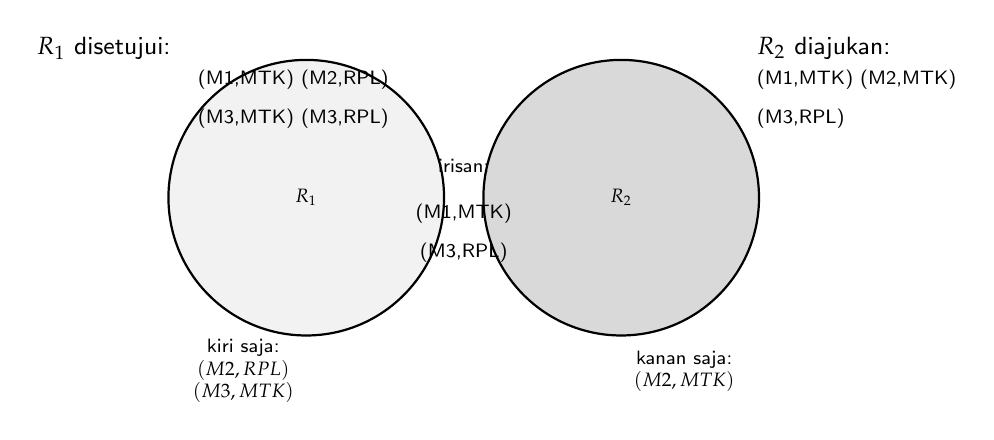
\begin{tikzpicture}[
			circ/.style={circle, draw=black, thick, minimum size=3.5cm, align=center, font=\ttfamily\scriptsize},
			lbl/.style={font=\sffamily\small}
		]
		\begin{scope}[shift={(-2,0)}]
			\node[circ, fill=black!5] at (0,0) {$R_1$};
		\end{scope}
		\begin{scope}[shift={(2,0)}]
			\node[circ, fill=black!15] at (0,0) {$R_2$};
		\end{scope}
		\node[lbl, anchor=east] at (-3.6, 1.9) {$R_1$ disetujui:};
		\node[font=\scriptsize\sffamily, anchor=west] at (-3.5, 1.5) {(M1,MTK) (M2,RPL)};
		\node[font=\scriptsize\sffamily, anchor=west] at (-3.5, 1.0) {(M3,MTK) (M3,RPL)};
		\node[lbl, anchor=west] at (3.6, 1.9) {$R_2$ diajukan:};
		\node[font=\scriptsize\sffamily, anchor=west] at (3.6, 1.5) {(M1,MTK) (M2,MTK)};
		\node[font=\scriptsize\sffamily, anchor=west] at (3.6, 1.0) {(M3,RPL)};
		\node[font=\scriptsize\sffamily, align=center] at (0, 0.4) {irisan:};
		\node[font=\scriptsize\sffamily, align=center] at (0, -0.2) {(M1,MTK)};
		\node[font=\scriptsize\sffamily, align=center] at (0, -0.7) {(M3,RPL)};
		\node[font=\scriptsize\sffamily, align=center] at (-2.8, -2.2) {kiri saja:\\$(M2,RPL)$\\$(M3,MTK)$};
		\node[font=\scriptsize\sffamily, align=center] at (2.8, -2.2) {kanan saja:\\$(M2,MTK)$};
	\end{tikzpicture}
	\caption{Diagram Venn kombinasi $R_1$ dan $R_2$ dengan daerah irisan dan selisih.}
	\label{fig:kombinasi}
\end{figure}

Cara membaca Gambar~\ref{fig:kombinasi}: gambar ini menampilkan dua lingkaran yang saling berpotongan di tengah. Lingkaran kiri berlabel $R_1$ mewakili pasangan yang disetujui, dengan latar abu-abu sangat muda. Lingkaran kanan berlabel $R_2$ mewakili pasangan yang diajukan, dengan latar abu-abu yang lebih gelap. Di sebelah kiri tertulis daftar anggota $R_1$, di sebelah kanan tertulis daftar anggota $R_2$. Di daerah irisan tengah tertulis $(M1,MTK)$ dan $(M3,RPL)$ yang ada di kedua himpunan. Di bawah kiri tertulis "kiri saja" dengan $(M2,RPL)$ dan $(M3,MTK)$ yang hanya ada di $R_1$. Di bawah kanan tertulis "kanan saja" dengan $(M2,MTK)$ yang hanya ada di $R_2$. Inti pesan gambar ini adalah kombinasi relasi memilah pasangan berdasarkan kehadirannya di satu atau kedua relasi.

\subsection{Mengapa Ini Penting}

Di portal KRS, kombinasi relasi dipakai untuk audit dan pelaporan. Irisan dipakai untuk menampilkan pasangan yang sudah lengkap prosesnya. Gabungan dipakai untuk menampilkan seluruh riwayat pengajuan. Selisih dipakai untuk mendeteksi anomali, misalnya pasangan yang disetujui tanpa pernah diajukan. Beda simetris dipakai untuk menampilkan pasangan yang perlu diperiksa manual. Tanpa konsep kombinasi, setiap audit memerlukan query khusus yang ditulis dari awal \cite{date}.

\subsection{Ringkasan}

Tabel~\ref{tab:kombinasi} merangkum empat operasi kombinasi.

\begin{table}[H]
	\centering
	\caption{Ringkasan kombinasi relasi dalam konteks KRS.}
	\label{tab:kombinasi}
	\small
	\begin{tabularx}{\textwidth}{l X X}
		\toprule
		Operasi          & Hasil                        & Arti di KRS                     \\
		\midrule
		$R_1 \cap R_2$   & $(M1,MTK),(M3,RPL)$          & diajukan dan disetujui          \\
		$R_1 \cup R_2$   & lima pasangan                & pernah diajukan atau disetujui  \\
		$R_1-R_2$        & $(M2,RPL),(M3,MTK)$          & disetujui tanpa diajukan        \\
		$R_2-R_1$        & $(M2,MTK)$                   & diajukan tetapi tidak disetujui \\
		$R_1 \oplus R_2$ & $(M2,MTK),(M2,RPL),(M3,MTK)$ & hanya di salah satu             \\
		\bottomrule
	\end{tabularx}
\end{table}

\section{Komposisi Relasi}

\subsection{Analogi: Rantai Jawaban Bertingkat}

Pertanyaan portal KRS bisa bertingkat. Pertama: "Siapa mengambil MTK?" Jawabannya M1 dan M3. Kedua: "Siapa dosen pengampu MTK?" Jawabannya D1. Jika kedua jawaban dirangkai, portal bisa menjawab pertanyaan gabungan: "Siapa dosen M1?" Jawabannya D1.

Rantai itu melewati tiga himpunan: mahasiswa, mata kuliah, dan dosen. Relasi pertama menghubungkan mahasiswa ke mata kuliah. Relasi kedua menghubungkan mata kuliah ke dosen. Hasil gabungannya menghubungkan mahasiswa langsung ke dosen, melewati mata kuliah di tengah.

Hasil gabungan itulah komposisi relasi.

\subsection{Definisi Formal}

Misalkan $R$ adalah relasi dari $A$ ke $B$ dan $S$ adalah relasi dari $B$ ke $C$. Komposisi $S \circ R$ adalah relasi dari $A$ ke $C$ yang berisi semua pasangan $(a,c)$ sedemikian sehingga ada $b \in B$ dengan $(a,b) \in R$ dan $(b,c) \in S$. Notasinya $S \circ R=\{(a,c) \mid a \in A, c \in C, \exists b \in B, (a,b) \in R, (b,c) \in S\}$ \cite{rosen}.

Perhatikan urutan penulisan. Komposisi ditulis $S \circ R$, bukan $R \circ S$. Urutannya dibaca dari kanan ke kiri, yaitu $R$ dikerjakan dulu, lalu $S$. Ini berbeda dari notasi fungsi biasa yang dibaca dari dalam ke luar.

\subsection{Contoh Berangka}

Misalkan $R$ adalah relasi dari $\{1,2,3\}$ ke $\{2,4,6,8\}$ yang berisi $\{(1,2),(1,6),(2,4),(3,4),(3,6),(3,8)\}$. Misalkan $S$ adalah relasi dari $\{2,4,6,8\}$ ke $\{s,t,u\}$ yang berisi $\{(2,u),(4,s),(4,t),(6,t),(8,u)\}$.

Untuk menghitung $S \circ R$, telusuri setiap pasangan di $R$ dan cari pasangan lanjutan di $S$. Proses penelusuran ini ditampilkan pada Tabel~\ref{tab:komposisi-langkah}.

\begin{table}[H]
	\centering
	\caption{Penelusuran langkah komposisi $S \circ R$.}
	\label{tab:komposisi-langkah}
	\small
	\begin{tabular}{c c c l}
		\toprule
		Dari $A$ & Via $B$ & Ke $C$  & Hasil                             \\
		\midrule
		1        & 2       & u       & $(1,u)$ ditambahkan               \\
		1        & 6       & t       & $(1,t)$ ditambahkan               \\
		2        & 4       & s dan t & $(2,s)$, $(2,t)$ ditambahkan      \\
		3        & 4       & s dan t & $(3,s)$, $(3,t)$ ditambahkan      \\
		3        & 6       & t       & $(3,t)$ sudah ada, tidak ditambah \\
		3        & 8       & u       & $(3,u)$ ditambahkan               \\
		\bottomrule
	\end{tabular}
\end{table}

Hasil akhirnya $S \circ R=\{(1,u),(1,t),(2,s),(2,t),(3,s),(3,t),(3,u)\}$. Ada tujuh pasangan di komposisi, walaupun $R$ berisi enam pasangan. Jumlahnya bertambah karena satu pasangan di $R$ bisa dilanjutkan dengan dua pasangan di $S$, misalnya $(2,4)$ dilanjutkan dengan $(4,s)$ dan $(4,t)$. Sebaliknya, $(3,t)$ muncul dua kali dari rantai berbeda, tetapi dihitung satu kali karena relasi adalah himpunan. Perhatikan Gambar~\ref{fig:komposisi}.

\begin{figure}[H]
	\centering
	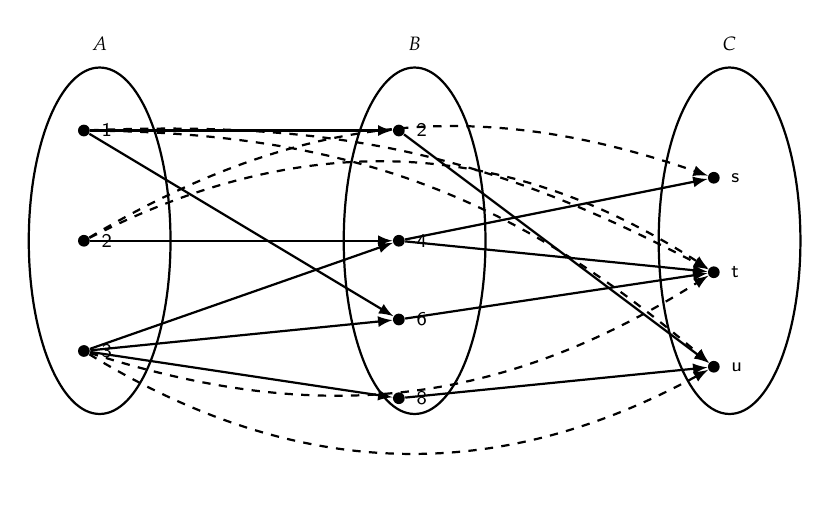
\begin{tikzpicture}[
			dot/.style={circle, fill=black, inner sep=1.5pt},
			elbl/.style={font=\scriptsize\sffamily}
		]
		\draw[thick] (-4, 0) ellipse (0.9 and 2.2);
		\draw[thick] (0, 0) ellipse (0.9 and 2.2);
		\draw[thick] (4, 0) ellipse (0.9 and 2.2);
		\node[elbl] at (-4, 2.5) {$A$};
		\node[elbl] at (0, 2.5) {$B$};
		\node[elbl] at (4, 2.5) {$C$};

		\node[dot] (n1) at (-4.2, 1.4) {};
		\node[dot] (n2) at (-4.2, 0) {};
		\node[dot] (n3) at (-4.2, -1.4) {};
		\node[elbl, anchor=west] at (-4.1, 1.4) {1};
		\node[elbl, anchor=west] at (-4.1, 0) {2};
		\node[elbl, anchor=west] at (-4.1, -1.4) {3};

		\node[dot] (b2) at (-0.2, 1.4) {};
		\node[dot] (b4) at (-0.2, 0) {};
		\node[dot] (b6) at (-0.2, -1.0) {};
		\node[dot] (b8) at (-0.2, -2.0) {};
		\node[elbl, anchor=west] at (-0.1, 1.4) {2};
		\node[elbl, anchor=west] at (-0.1, 0) {4};
		\node[elbl, anchor=west] at (-0.1, -1.0) {6};
		\node[elbl, anchor=west] at (-0.1, -2.0) {8};

		\node[dot] (c1) at (3.8, 0.8) {};
		\node[dot] (c2) at (3.8, -0.4) {};
		\node[dot] (c3) at (3.8, -1.6) {};
		\node[elbl, anchor=west] at (3.9, 0.8) {s};
		\node[elbl, anchor=west] at (3.9, -0.4) {t};
		\node[elbl, anchor=west] at (3.9, -1.6) {u};

		\draw[thick, -latex] (n1) -- (b2);
		\draw[thick, -latex] (n1) -- (b6);
		\draw[thick, -latex] (n2) -- (b4);
		\draw[thick, -latex] (n3) -- (b4);
		\draw[thick, -latex] (n3) -- (b6);
		\draw[thick, -latex] (n3) -- (b8);

		\draw[thick, -latex] (b2) -- (c3);
		\draw[thick, -latex] (b4) -- (c1);
		\draw[thick, -latex] (b4) -- (c2);
		\draw[thick, -latex] (b6) -- (c2);
		\draw[thick, -latex] (b8) -- (c3);

		\draw[thick, dashed, -latex, bend left=15] (n1) to (c2);
		\draw[thick, dashed, -latex, bend left=20] (n1) to (c3);
		\draw[thick, dashed, -latex, bend left=25] (n2) to (c1);
		\draw[thick, dashed, -latex, bend left=30] (n2) to (c2);
		\draw[thick, dashed, -latex, bend right=25] (n3) to (c2);
		\draw[thick, dashed, -latex, bend right=30] (n3) to (c3);
	\end{tikzpicture}
	\caption{Komposisi $S \circ R$: setiap rantai dua panah dipendekkan menjadi satu panah putus-putus.}
	\label{fig:komposisi}
\end{figure}

Cara membaca Gambar~\ref{fig:komposisi}: gambar ini menampilkan tiga elips berderet dari kiri ke kanan, berlabel $A$, $B$, dan $C$ di atas masing-masing. Elips $A$ berisi tiga titik berlabel 1, 2, 3 dari atas ke bawah. Elips $B$ berisi empat titik berlabel 2, 4, 6, 8 dari atas ke bawah. Elips $C$ berisi tiga titik berlabel s, t, u dari atas ke bawah. Panah penuh menghubungkan titik-titik di $A$ ke titik-titik di $B$ sesuai relasi $R$. Panah penuh lain menghubungkan titik-titik di $B$ ke titik-titik di $C$ sesuai relasi $S$. Panah putus-putus melengkung langsung dari titik-titik di $A$ ke titik-titik di $C$ sesuai komposisi $S \circ R$. Panah putus-putus adalah jalan pintas yang melewati $B$. Inti pesan gambar ini adalah komposisi memendekkan rantai dua langkah menjadi satu langkah.

\subsection{Cara Berpikir: Membaca Notasi Komposisi}

Saat membaca $S \circ R$, jangan dibaca dari kiri ke kanan seperti membaca buku. Bacalah dari kanan ke kiri. $R$ dikerjakan lebih dulu karena $R$ adalah relasi yang lebih dekat ke titik awal. $S$ dikerjakan setelahnya karena $S$ adalah relasi yang lebih dekat ke titik akhir.

Cara mudah mengingatnya: notasi $S \circ R$ dibaca "S setelah R". Kata "setelah" menandakan urutan pengerjaan. Yang disebut terakhir dikerjakan lebih dulu. Aturan ini sama dengan notasi komposisi fungsi pada matematika, dan sengaja dibuat konsisten agar pembaca yang sudah mengenal komposisi fungsi tidak bingung.

\subsection{Kalau Salah: Urutan Komposisi Dibaca Terbalik}

Kesalahan paling sering adalah membaca $S \circ R$ dari kiri ke kanan, sehingga mengira $R$ dikerjakan setelah $S$. Padahal notasi $S \circ R$ dibaca dari kanan ke kiri. $R$ dulu, baru $S$.

Akibatnya, jika himpunan tidak dirancang simetris, pengembang akan mencoba menyambung $S$ dulu baru $R$, padahal $S$ berakhir di $C$ dan $R$ dimulai dari $A$. Kedua ujung tidak bertemu, dan komposisi tidak terdefinisi.

Cara aman adalah membaca notasi dengan suara. "S setelah R" berarti kerjakan R dulu, lalu S. Kalau dibaca "S komposisi R", pengucapan itu juga menandakan urutan yang sama: R dulu.

\subsection{Mengapa Komposisi Penting}

Komposisi adalah dasar penyambungan tabel di basis data. Setiap kali pengembang menulis JOIN antara tabel Mahasiswa, KRS, dan Mata Kuliah, ia sedang melakukan komposisi relasi. JOIN Mahasiswa-KRS menghasilkan relasi antara mahasiswa dan mata kuliah. JOIN KRS-MataKuliah menghasilkan relasi antara mahasiswa dan mata kuliah lagi, tetapi dengan detail mata kuliah. Kedua JOIN itu berantai seperti komposisi.

Memahami komposisi membantu pengembang menjelaskan mengapa query yang menyambung tiga tabel lebih lambat daripada query dua tabel. Setiap sambungan menambah rantai yang harus ditelusuri \cite{silberschatz}.

\subsection{Ringkasan}

Tabel~\ref{tab:komposisi} merangkum komposisi relasi.

\begin{table}[H]
	\centering
	\caption{Ringkasan komposisi relasi.}
	\label{tab:komposisi}
	\small
	\begin{tabularx}{\textwidth}{l X}
		\toprule
		Aspek       & Isi                                                                       \\
		\midrule
		Notasi      & $S \circ R$                                                               \\
		Urutan baca & dari kanan ke kiri ($R$ dulu)                                             \\
		Syarat      & kodomain $R$ = domain $S$                                                 \\
		Definisi    & $(a,c) \in S \circ R$ jika ada $b$ dengan $(a,b) \in R$ dan $(b,c) \in S$ \\
		Hasil       & relasi dari domain $R$ ke kodomain $S$                                    \\
		Padanan SQL & JOIN berantai                                                             \\
		\bottomrule
	\end{tabularx}
\end{table}

\section{Sintesis Seluruh Konsep}

Tabel~\ref{tab:sintesis} menyandingkan seluruh konsep dalam satu pandangan.

\begin{table}[H]
	\centering
	\caption{Sintesis konsep relasi untuk rekayasa perangkat lunak.}
	\label{tab:sintesis}
	\footnotesize
	\begin{tabularx}{\textwidth}{l X X X}
		\toprule
		Lapisan      & Pertanyaan                             & Alat                             & Contoh penerapan                \\
		\midrule
		Bahan        & kemungkinan pasangan apa yang ada      & $A \times B$                     & daftar seluruh kombinasi KRS    \\
		Definisi     & pasangan mana yang benar-benar terjadi & $R \subseteq A \times B$         & isi tabel KRS                   \\
		Representasi & bagaimana pasangan disajikan           & diagram, tabel, matriks          & tampilan portal                 \\
		Sifat        & hubungan seperti apa yang terbentuk    & refleksif, menghantar, setangkup & validasi integritas             \\
		Invers       & pertanyaan dari arah sebaliknya        & $R^{-1}$                         & "siapa mengambil MTK"           \\
		Kombinasi    & memilah pasangan                       & $\cap, \cup, -, \oplus$          & filter pengajuan vs persetujuan \\
		Komposisi    & menyambung dua rantai                  & $S \circ R$                      & "siapa dosen M1"                \\
		\bottomrule
	\end{tabularx}
\end{table}

Sintesis dari Tabel~\ref{tab:sintesis} adalah satu pola berpikir. Data mentah berupa pasangan diubah menjadi relasi. Relasi disajikan dalam tiga cara. Sifatnya diperiksa untuk memastikan konsistensi. Pertanyaan balik dijawab dengan invers. Pertanyaan berantai dijawab dengan komposisi. Pola ini berlaku dari sistem KRS sampai sistem rekomendasi.

\section{Studi Kasus: Sistem Akademik Sederhana}

\subsection{Langkah 1: Definisikan Himpunan}

Tiga himpunan yang terlibat adalah Mahasiswa $M=\{M1,M2,M3\}$, Mata Kuliah $K=\{\text{MTK, RPL}\}$, dan Dosen $D=\{D1,D2\}$. Setiap himpunan berisi elemen berbeda tanpa duplikat. Ketiga himpunan ini adalah dasar dari seluruh perhitungan berikutnya.

\subsection{Langkah 2: Bentuk Perkalian Kartesian}

Perkalian kartesian $M \times K$ berisi enam pasangan: $(M1,MTK)$, $(M1,RPL)$, $(M2,MTK)$, $(M2,RPL)$, $(M3,MTK)$, $(M3,RPL)$. Inilah semua kemungkinan hubungan antara mahasiswa dan mata kuliah. Setiap pasangan adalah satu kemungkinan yang boleh terjadi, tetapi tidak semua kemungkinan benar-benar terjadi.

\subsection{Langkah 3: Definisikan Relasi Mengambil}

Relasi $R_1$ adalah himpunan bagian dari $M \times K$ yang berisi pasangan yang benar-benar diambil semester ini. Isinya $R_1=\{(M1,MTK),(M2,RPL),(M3,MTK),(M3,RPL)\}$. Dari enam kemungkinan, hanya empat yang terjadi. Pasangan $(M1,RPL)$ dan $(M2,MTK)$ tidak termasuk karena kedua mahasiswa itu tidak mengambil kedua mata kuliah tersebut.

\subsection{Langkah 4: Representasikan sebagai Matriks Biner}

Susun matriks biner dengan baris untuk M1, M2, M3 dan kolom untuk MTK, RPL. Matriksnya adalah $\begin{bmatrix}1&0\\0&1\\1&1\end{bmatrix}$. Baris pertama untuk M1: mengambil MTK tetapi tidak RPL. Baris kedua untuk M2: tidak MTK tetapi RPL. Baris ketiga untuk M3: keduanya. Jumlah angka 1 pada matriks adalah empat, cocok dengan kardinalitas $R_1$.

\subsection{Langkah 5: Tentukan Relasi Invers}

Invers $R_1^{-1}$ adalah relasi dari $K$ ke $M$ yang berisi pasangan $(MTK,M1)$, $(RPL,M2)$, $(MTK,M3)$, dan $(RPL,M3)$. Dengan kata lain, MTK diambil oleh M1 dan M3, sedangkan RPL diambil oleh M2 dan M3. Matriks binernya adalah transpos dari matriks sebelumnya, yaitu $\begin{bmatrix}1&0&1\\0&1&1\end{bmatrix}$.

\subsection{Langkah 6: Definisikan Relasi Mengampu}

Relasi $R_2$ dari $K$ ke $D$ berisi pasangan $(MTK,D1)$ dan $(RPL,D2)$. Setiap mata kuliah diampu oleh tepat satu dosen, sehingga setiap baris di $R_2$ punya satu pasangan. Relasi ini adalah fungsi dari $K$ ke $D$, karena setiap elemen $K$ punya tepat satu pasangan di $D$.

\subsection{Langkah 7: Hitung Komposisi}

Komposisi $R_2 \circ R_1$ berisi pasangan antara mahasiswa dan dosen. Setiap pasangan $(m,k)$ di $R_1$ disambung dengan $(k,d)$ di $R_2$. Pasangan $(M1,MTK)$ disambung dengan $(MTK,D1)$ menjadi $(M1,D1)$. Pasangan $(M2,RPL)$ disambung dengan $(RPL,D2)$ menjadi $(M2,D2)$. Pasangan $(M3,MTK)$ menjadi $(M3,D1)$. Pasangan $(M3,RPL)$ menjadi $(M3,D2)$.

Hasilnya $R_2 \circ R_1=\{(M1,D1),(M2,D2),(M3,D1),(M3,D2)\}$. M1 diajar D1, M2 diajar D2, M3 diajar kedua dosen karena mengambil dua mata kuliah.

\subsection{Langkah 8: Verifikasi Jawaban}

Portal KRS harus menjawab pertanyaan "siapa dosen M3" dengan dua nama, yaitu D1 dan D2. Jawaban itu berasal dari komposisi, bukan dari tabel baru. Data mentahnya tetap hanya $R_1$ dan $R_2$. Portal menghitung komposisi pada saat ada permintaan, tanpa menyimpannya kembali. Inilah sikap yang diuji kasus ini: data hanya disimpan sekali, jawaban turunan dihitung ketika diperlukan \cite{silberschatz}. Alur langkah studi kasus ditunjukkan pada Gambar~\ref{fig:alur-studi-kasus}.

\begin{figure}[H]
	\centering
	\begin{tikzpicture}[
			step/.style={rectangle, draw=black, thick, fill=black!5, text width=9cm, align=left, minimum height=0.7cm, font=\sffamily\small, inner sep=8pt},
			line/.style={draw, thick, -latex}
		]
		\node[step] (s1) {\textbf{1.} Definisikan himpunan $M$, $K$, $D$};
		\node[step, below=0.25cm of s1] (s2) {\textbf{2.} Bentuk $M \times K$};
		\node[step, below=0.25cm of s2] (s3) {\textbf{3.} Definisikan $R_1$ mengambil};
		\node[step, below=0.25cm of s3] (s4) {\textbf{4.} Representasikan $R_1$ sebagai matriks biner};
		\node[step, below=0.25cm of s4] (s5) {\textbf{5.} Hitung invers $R_1^{-1}$};
		\node[step, below=0.25cm of s5] (s6) {\textbf{6.} Definisikan $R_2$ mengampu};
		\node[step, below=0.25cm of s6] (s7) {\textbf{7.} Hitung komposisi $R_2 \circ R_1$};
		\node[step, below=0.25cm of s7] (s8) {\textbf{8.} Verifikasi jawaban portal};
		\draw[line] (s1) -- (s2);
		\draw[line] (s2) -- (s3);
		\draw[line] (s3) -- (s4);
		\draw[line] (s4) -- (s5);
		\draw[line] (s5) -- (s6);
		\draw[line] (s6) -- (s7);
		\draw[line] (s7) -- (s8);
	\end{tikzpicture}
	\caption{Alur delapan langkah studi kasus sistem akademik.}
	\label{fig:alur-studi-kasus}
\end{figure}

Cara membaca Gambar~\ref{fig:alur-studi-kasus}: gambar ini menampilkan delapan kotak persegi panjang tersusun dari atas ke bawah. Setiap kotak berisi satu langkah, diawali angka tebal. Kotak pertama berisi "Definisikan himpunan M, K, D". Kotak kedua berisi "Bentuk M × K". Kotak ketiga berisi "Definisikan R1 mengambil". Kotak keempat berisi "Representasikan R1 sebagai matriks biner". Kotak kelima berisi "Hitung invers R1^-1". Kotak keenam berisi "Definisikan R2 mengampu". Kotak ketujuh berisi "Hitung komposisi R2 ∘ R1". Kotak kedelapan berisi "Verifikasi jawaban portal". Setiap kotak dihubungkan ke kotak berikutnya oleh panah pendek yang mengarah ke bawah. Latar kotak abu-abu sangat muda. Inti pesan gambar ini adalah proses pemodelan KRS berjalan berurutan dari definisi himpunan sampai verifikasi.

\begin{table}[H]
	\centering
	\caption{Ringkasan hasil studi kasus sistem akademik.}
	\label{tab:studi-kasus}
	\small
	\begin{tabularx}{\textwidth}{l X l}
		\toprule
		Langkah & Operasi                 & Hasil                                               \\
		\midrule
		1       & himpunan $M$, $K$, $D$  & 3, 2, 2 elemen                                      \\
		2       & $M \times K$            & 6 pasangan                                          \\
		3       & $R_1$ mengambil         & 4 pasangan                                          \\
		4       & matriks biner $R_1$     & $\begin{smallmatrix}1&0\\0&1\\1&1\end{smallmatrix}$ \\
		5       & $R_1^{-1}$ diambil oleh & 4 pasangan                                          \\
		6       & $R_2$ mengampu          & 2 pasangan                                          \\
		7       & $R_2 \circ R_1$         & 4 pasangan mahasiswa-dosen                          \\
		8       & verifikasi              & data tersimpan sekali, jawaban dihitung             \\
		\bottomrule
	\end{tabularx}
\end{table}

\section{Kesalahan Umum dan Cara Menghindarinya}

Tabel~\ref{tab:kesalahan} memuat kesalahan yang paling sering muncul saat bekerja dengan relasi.

\begin{table}[H]
	\centering
	\caption{Kesalahan umum pada penerapan teori relasi.}
	\label{tab:kesalahan}
	\footnotesize
	\begin{tabularx}{\textwidth}{l X X}
		\toprule
		Kesalahan                                        & Akibat                      & Perbaikan                          \\
		\midrule
		mengira $A \times B=B \times A$                  & urutan komponen tertukar    & komponen pertama dari $A$          \\
		mengira $|A \times B|=|A|+|B|$                   & kardinalitas salah          & gunakan $|A| \cdot |B|$            \\
		menyimpan setiap kombinasi kartesian             & tabel membengkak            & simpan hanya pasangan yang terjadi \\
		matriks biner diperlakukan matriks biasa         & determinan tidak bermakna   & baca posisi 1 saja                 \\
		mengira tidak setangkup $=$ tolak-setangkup      & validasi longgar            & periksa dua sifat terpisah         \\
		setangkup tanpa memeriksa diagonal               & refleksif terlewat          & cek diagonal utama                 \\
		invers relasi dihitung dengan rumus matriks      & hasil salah                 & balik pasangan saja                \\
		urutan komposisi dibaca kiri ke kanan            & komposisi tidak terdefinisi & baca $S \circ R$ dari kanan        \\
		komposisi disimpan sebagai tabel baru            & data ganda                  & hitung saat diperlukan             \\
		representasi diagram panah dipakai di basis data & tidak terbaca mesin         & pakai tabel atau matriks           \\
		\bottomrule
	\end{tabularx}
\end{table}

Dua kesalahan yang paling sering adalah mengira tidak setangkup sama dengan tolak-setangkup, dan menyimpan hasil komposisi sebagai tabel baru. Kesalahan pertama membuat validasi longgar. Kesalahan kedua membuat data menjadi ganda, dan setiap kali data asli berubah, salinan lama tidak ikut berubah. Keduanya dapat dicegah dengan memeriksa sifat secara terpisah dan menyimpan data hanya sekali.

\section{Lembar Rujukan Cepat}

Tabel~\ref{tab:rujukan-cepat} adalah lembar rujukan untuk ujian atau kerja. Baris pertama sampai baris terakhir mencakup seluruh notasi yang dipakai di modul ini.

\begin{table}[H]
	\centering
	\caption{Lembar rujukan cepat teori relasi.}
	\label{tab:rujukan-cepat}
	\footnotesize
	\begin{tabularx}{\textwidth}{l X}
		\toprule
		Kebutuhan               & Notasi atau langkah                                            \\
		\midrule
		perkalian kartesian     & $A \times B=\{(a,b) \mid a \in A, b \in B\}$                   \\
		kardinalitas kartesian  & $|A \times B|=|A| \cdot |B|$                                   \\
		definisi relasi         & $R \subseteq A \times B$                                       \\
		representasi diagram    & panah dari asal ke tujuan                                      \\
		representasi tabel      & kolom $A$ dan kolom $B$                                        \\
		representasi matriks    & $m_{ij}=1$ jika $(a_i,b_j) \in R$                              \\
		sifat refleksif         & $(a,a) \in R$ untuk semua $a$                                  \\
		sifat menghantar        & $(a,b),(b,c) \in R \Rightarrow (a,c) \in R$                    \\
		sifat setangkup         & $(a,b) \in R \Rightarrow (b,a) \in R$                          \\
		sifat tolak-setangkup   & $(a,b),(b,a) \in R \Rightarrow a=b$                            \\
		invers relasi           & $R^{-1}=\{(b,a) \mid (a,b) \in R\}$                            \\
		matriks invers relasi   & $M^T$ bukan $M^{-1}$                                           \\
		kombinasi irisan        & $R_1 \cap R_2$                                                 \\
		kombinasi gabungan      & $R_1 \cup R_2$                                                 \\
		kombinasi selisih       & $R_1-R_2$                                                      \\
		kombinasi beda simetris & $R_1 \oplus R_2$                                               \\
		komposisi               & $S \circ R=\{(a,c) \mid \exists b, (a,b) \in R, (b,c) \in S\}$ \\
		urutan komposisi        & dibaca dari kanan ke kiri                                      \\
		\bottomrule
	\end{tabularx}
\end{table}

\section{Kesimpulan}

Modul ini menunjukkan bahwa relasi adalah alat kerja untuk mengubah data berpasangan menjadi model yang dapat diperiksa dan ditelusuri. Tiga prinsip penutup adalah sebagai berikut.

\begin{enumerate}
	\item Nyatakan relasi sebagai subset dari perkalian kartesian. Tanpa menyebut domain dan kodomain, pasangan apa pun bisa tampak sah padahal tidak terdefinisi.
	\item Jangan simpan jawaban turunan. Invers dan komposisi dihitung dari data asli saat diperlukan. Menyimpannya sebagai tabel baru membuat data ganda dan tidak konsisten ketika data asli berubah.
	\item Periksa keempat sifat secara terpisah. Refleksif, menghantar, setangkup, dan tolak-setangkup adalah empat pemeriksaan yang berbeda. Menggabungkan dua di antaranya menjadi satu adalah sumber kesalahan yang paling sering.
\end{enumerate}

Dengan tiga prinsip itu, pembaca dapat memodelkan hubungan antar entitas menjadi relasi, menyajikannya dengan cara yang sesuai, memeriksa sifatnya untuk menjaga integritas, serta menjawab pertanyaan arah sebaliknya dan pertanyaan berantai tanpa menyimpan data ganda.

\newpage
\section*{Referensi}
\addcontentsline{toc}{section}{Referensi}

\begin{thebibliography}{99}

	\bibitem{rosen}
	Rosen, K. H. (2019).
	\textit{Discrete Mathematics and Its Applications} (8th ed.).
	McGraw-Hill Education.

	\bibitem{munir}
	Munir, R. (2012).
	\textit{Matematika Diskrit}.
	Informatika.

	\bibitem{epp}
	Epp, S. S. (2010).
	\textit{Discrete Mathematics with Applications} (4th ed.).
	Brooks Cole.

	\bibitem{lipschutz}
	Lipschutz, S., \& Lipson, M. (2007).
	\textit{Discrete Mathematics}.
	McGraw-Hill.

	\bibitem{silberschatz}
	Silberschatz, A., Korth, H. F., \& Sudarshan, S. (2019).
	\textit{Database System Concepts} (7th ed.).
	McGraw-Hill Education.

	\bibitem{kleppmann}
	Kleppmann, M. (2017).
	\textit{Designing Data-Intensive Applications}.
	O'Reilly Media.

	\bibitem{sommerville}
	Sommerville, I. (2016).
	\textit{Software Engineering} (10th ed.).
	Pearson.

	\bibitem{date}
	Date, C. J. (2003).
	\textit{An Introduction to Database Systems} (8th ed.).
	Addison-Wesley.

\end{thebibliography}

\end{document}
